
%% bare_jrnl.tex
%% V1.4b
%% 2015/08/26
%% by Michael Shell
%% see http://www.michaelshell.org/
%% for current contact information.
%%
%% This is a skeleton file demonstrating the use of IEEEtran.cls
%% (requires IEEEtran.cls version 1.8b or later) with an IEEE
%% journal paper.
%%
%% Support sites:
%% http://www.michaelshell.org/tex/ieeetran/
%% http://www.ctan.org/pkg/ieeetran
%% and
%% http://www.ieee.org/

%%*************************************************************************
%% Legal Notice:
%% This code is offered as-is without any warranty either expressed or
%% implied; without even the implied warranty of MERCHANTABILITY or
%% FITNESS FOR A PARTICULAR PURPOSE! 
%% User assumes all risk.
%% In no event shall the IEEE or any contributor to this code be liable for
%% any damages or losses, including, but not limited to, incidental,
%% consequential, or any other damages, resulting from the use or misuse
%% of any information contained here.
%%
%% All comments are the opinions of their respective authors and are not
%% necessarily endorsed by the IEEE.
%%
%% This work is distributed under the LaTeX Project Public License (LPPL)
%% ( http://www.latex-project.org/ ) version 1.3, and may be freely used,
%% distributed and modified. A copy of the LPPL, version 1.3, is included
%% in the base LaTeX documentation of all distributions of LaTeX released
%% 2003/12/01 or later.
%% Retain all contribution notices and credits.
%% ** Modified files should be clearly indicated as such, including  **
%% ** renaming them and changing author support contact information. **
%%*************************************************************************


% *** Authors should verify (and, if needed, correct) their LaTeX system  ***
% *** with the testflow diagnostic prior to trusting their LaTeX platform ***
% *** with production work. The IEEE's font choices and paper sizes can   ***
% *** trigger bugs that do not appear when using other class files.       ***                          ***
% The testflow support page is at:
% http://www.michaelshell.org/tex/testflow/



\documentclass[10pt,journal]{article}
%
% If IEEEtran.cls has not been installed into the LaTeX system files,
% manually specify the path to it like:
% \documentclass[journal]{../sty/IEEEtran}


% Some very useful LaTeX packages include:
% (uncomment the ones you want to load)


% *** MISC UTILITY PACKAGES ***
%
%\usepackage{ifpdf}
% Heiko Oberdiek's ifpdf.sty is very useful if you need conditional
% compilation based on whether the output is pdf or dvi.
% usage:
% \ifpdf
%   % pdf code
% \else
%   % dvi code
% \fi
% The latest version of ifpdf.sty can be obtained from:
% http://www.ctan.org/pkg/ifpdf
% Also, note that IEEEtran.cls V1.7 and later provides a builtin
% \ifCLASSINFOpdf conditional that works the same way.
% When switching from latex to pdflatex and vice-versa, the compiler may
% have to be run twice to clear warning/error messages.






% *** CITATION PACKAGES ***
%
\usepackage{cite}
% cite.sty was written by Donald Arseneau
% V1.6 and later of IEEEtran pre-defines the format of the cite.sty package
% \cite{} output to follow that of the IEEE. Loading the cite package will
% result in citation numbers being automatically sorted and properly
% "compressed/ranged". e.g., [1], [9], [2], [7], [5], [6] without using
% cite.sty will become [1], [2], [5]--[7], [9] using cite.sty. cite.sty's
% \cite will automatically add leading space, if needed. Use cite.sty's
% noadjust option (cite.sty V3.8 and later) if you want to turn this off
% such as if a citation ever needs to be enclosed in parenthesis.
% cite.sty is already installed on most LaTeX systems. Be sure and use
% version 5.0 (2009-03-20) and later if using hyperref.sty.
% The latest version can be obtained at:
% http://www.ctan.org/pkg/cite
% The documentation is contained in the cite.sty file itself.



\usepackage{algorithm}
\usepackage{algpseudocode}
\makeatletter 
\renewcommand\thealgorithm{\thesection.\arabic{algorithm}} 
\@addtoreset{algorithm}{section} 
\makeatother

% *** GRAPHICS RELATED PACKAGES ***
%
%\ifCLASSINFOpdf
  \usepackage[pdftex]{graphicx}
  % declare the path(s) where your graphic files are
  % \graphicspath{{../pdf/}{../jpeg/}}
  % and their extensions so you won't have to specify these with
  % every instance of \includegraphics
  % \DeclareGraphicsExtensions{.pdf,.jpeg,.png}
%\else
  % or other class option (dvipsone, dvipdf, if not using dvips). graphicx
  % will default to the driver specified in the system graphics.cfg if no
  % driver is specified.
  % \usepackage[dvips]{graphicx}
  % declare the path(s) where your graphic files are
  % \graphicspath{{../eps/}}
  % and their extensions so you won't have to specify these with
  % every instance of \includegraphics
  % \DeclareGraphicsExtensions{.eps}
%\fi
% % graphicx was written by David Carlisle and Sebastian Rahtz. It is
% % required if you want graphics, photos, etc. graphicx.sty is already
% % installed on most LaTeX systems. The latest version and documentation
% % can be obtained at: 
% % http://www.ctan.org/pkg/graphicx
% % Another good source of documentation is "Using Imported Graphics in
% % LaTeX2e" by Keith Reckdahl which can be found at:
% % http://www.ctan.org/pkg/epslatex
% %
% % latex, and pdflatex in dvi mode, support graphics in encapsulated
% % postscript (.eps) format. pdflatex in pdf mode supports graphics
% % in .pdf, .jpeg, .png and .mps (metapost) formats. Users should ensure
% % that all non-photo figures use a vector format (.eps, .pdf, .mps) and
% % not a bitmapped formats (.jpeg, .png). The IEEE frowns on bitmapped formats
% % which can result in "jaggedy"/blurry rendering of lines and letters as
% % well as large increases in file sizes.
% %
% % You can find documentation about the pdfTeX application at:
% % http://www.tug.org/applications/pdftex





% *** MATH PACKAGES ***
%
% \usepackage{amsmath}
\usepackage{mathtools} %includes and extends `amsmath'. Needed for dcases
% A popular package from the American Mathematical Society that provides
% many useful and powerful commands for dealing with mathematics.
%
% Note that the amsmath package sets \interdisplaylinepenalty to 10000
% thus preventing page breaks from occurring within multiline equations. Use:
\interdisplaylinepenalty=2500
% after loading amsmath to restore such page breaks as IEEEtran.cls normally
% does. amsmath.sty is already installed on most LaTeX systems. The latest
% version and documentation can be obtained at:
% http://www.ctan.org/pkg/amsmath

\usepackage{blkarray, bigstrut} %
\usepackage{kbordermatrix}% http://www.hss.caltech.edu/~kcb/TeX/kbordermatrix.sty
% *** SPECIALIZED LIST PACKAGES ***
%
\usepackage{algorithm}
\usepackage{algpseudocode}
% algorithmic.sty was written by Peter Williams and Rogerio Brito.
% This package provides an algorithmic environment fo describing algorithms.
% You can use the algorithmic environment in-text or within a figure
% environment to provide for a floating algorithm. Do NOT use the algorithm
% floating environment provided by algorithm.sty (by the same authors) or
% algorithm2e.sty (by Christophe Fiorio) as the IEEE does not use dedicated
% algorithm float types and packages that provide these will not provide
% correct IEEE style captions. The latest version and documentation of
% algorithmic.sty can be obtained at:
% http://www.ctan.org/pkg/algorithms
% Also of interest may be the (relatively newer and more customizable)
% algorithmicx.sty package by Szasz Janos:
% http://www.ctan.org/pkg/algorithmicx




% *** ALIGNMENT PACKAGES ***
%
\usepackage{array}
% Frank Mittelbach's and David Carlisle's array.sty patches and improves
% the standard LaTeX2e array and tabular environments to provide better
% appearance and additional user controls. As the default LaTeX2e table
% generation code is lacking to the point of almost being broken with
% respect to the quality of the end results, all users are strongly
% advised to use an enhanced (at the very least that provided by array.sty)
% set of table tools. array.sty is already installed on most systems. The
% latest version and documentation can be obtained at:
% http://www.ctan.org/pkg/array


% IEEEtran contains the IEEEeqnarray family of commands that can be used to
% generate multiline equations as well as matrices, tables, etc., of high
% quality.




% *** SUBFIGURE PACKAGES ***
%\ifCLASSOPTIONcompsoc
 \usepackage[caption=false,font=normalsize,labelfont=sf,textfont=sf,position=top]{subfig}
%\else
 %\usepackage[caption=false,font=footnotesize]{subfig}
%\fi
% subfig.sty, written by Steven Douglas Cochran, is the modern replacement
% for subfigure.sty, the latter of which is no longer maintained and is
% incompatible with some LaTeX packages including fixltx2e. However,
% subfig.sty requires and automatically loads Axel Sommerfeldt's caption.sty
% which will override IEEEtran.cls' handling of captions and this will result
% in non-IEEE style figure/table captions. To prevent this problem, be sure
% and invoke subfig.sty's "caption=false" package option (available since
% subfig.sty version 1.3, 2005/06/28) as this is will preserve IEEEtran.cls
% handling of captions.
% Note that the Computer Society format requires a larger sans serif font
% than the serif footnote size font used in traditional IEEE formatting
% and thus the need to invoke different subfig.sty package options depending
% on whether compsoc mode has been enabled.
%
% The latest version and documentation of subfig.sty can be obtained at:
% http://www.ctan.org/pkg/subfig




% *** FLOAT PACKAGES ***
%
% \usepackage{fixltx2e}
% fixltx2e, the successor to the earlier fix2col.sty, was written by
% Frank Mittelbach and David Carlisle. This package corrects a few problems
% in the LaTeX2e kernel, the most notable of which is that in current
% LaTeX2e releases, the ordering of single and double column floats is not
% guaranteed to be preserved. Thus, an unpatched LaTeX2e can allow a
% single column figure to be placed prior to an earlier double column
% figure.
% Be aware that LaTeX2e kernels dated 2015 and later have fixltx2e.sty's
% corrections already built into the system in which case a warning will
% be issued if an attempt is made to load fixltx2e.sty as it is no longer
% needed.
% The latest version and documentation can be found at:
% http://www.ctan.org/pkg/fixltx2e
\usepackage{epstopdf}

\usepackage{stfloats}
% stfloats.sty was written by Sigitas Tolusis. This package gives LaTeX2e
% the ability to do double column floats at the bottom of the page as well
% as the top. (e.g., "\begin{figure*}[!b]" is not normally possible in
% LaTeX2e). It also provides a command:
%\fnbelowfloat
% to enable the placement of footnotes below bottom floats (the standard
% LaTeX2e kernel puts them above bottom floats). This is an invasive package
% which rewrites many portions of the LaTeX2e float routines. It may not work
% with other packages that modify the LaTeX2e float routines. The latest
% version and documentation can be obtained at:
% http://www.ctan.org/pkg/stfloats
% Do not use the stfloats baselinefloat ability as the IEEE does not allow
% \baselineskip to stretch. Authors submitting work to the IEEE should note
% that the IEEE rarely uses double column equations and that authors should try
% to avoid such use. Do not be tempted to use the cuted.sty or midfloat.sty
% packages (also by Sigitas Tolusis) as the IEEE does not format its papers in
% such ways.
% Do not attempt to use stfloats with fixltx2e as they are incompatible.
% Instead, use Morten Hogholm'a dblfloatfix which combines the features
% of both fixltx2e and stfloats:
%
% \usepackage{dblfloatfix}
% The latest version can be found at:
% http://www.ctan.org/pkg/dblfloatfix




%\ifCLASSOPTIONcaptionsoff
%  \usepackage[nomarkers]{endfloat}
% \let\MYoriglatexcaption\caption
% \renewcommand{\caption}[2][\relax]{\MYoriglatexcaption[#2]{#2}}
%\fi
% endfloat.sty was written by James Darrell McCauley, Jeff Goldberg and 
% Axel Sommerfeldt. This package may be useful when used in conjunction with 
% IEEEtran.cls'  captionsoff option. Some IEEE journals/societies require that
% submissions have lists of figures/tables at the end of the paper and that
% figures/tables without any captions are placed on a page by themselves at
% the end of the document. If needed, the draftcls IEEEtran class option or
% \CLASSINPUTbaselinestretch interface can be used to increase the line
% spacing as well. Be sure and use the nomarkers option of endfloat to
% prevent endfloat from "marking" where the figures would have been placed
% in the text. The two hack lines of code above are a slight modification of
% that suggested by in the endfloat docs (section 8.4.1) to ensure that
% the full captions always appear in the list of figures/tables - even if
% the user used the short optional argument of \caption[]{}.
% IEEE papers do not typically make use of \caption[]'s optional argument,
% so this should not be an issue. A similar trick can be used to disable
% captions of packages such as subfig.sty that lack options to turn off
% the subcaptions:
% For subfig.sty:
% \let\MYorigsubfloat\subfloat
% \renewcommand{\subfloat}[2][\relax]{\MYorigsubfloat[]{#2}}
% However, the above trick will not work if both optional arguments of
% the \subfloat command are used. Furthermore, there needs to be a
% description of each subfigure *somewhere* and endfloat does not add
% subfigure captions to its list of figures. Thus, the best approach is to
% avoid the use of subfigure captions (many IEEE journals avoid them anyway)
% and instead reference/explain all the subfigures within the main caption.
% The latest version of endfloat.sty and its documentation can obtained at:
% http://www.ctan.org/pkg/endfloat
%
% The IEEEtran \ifCLASSOPTIONcaptionsoff conditional can also be used
% later in the document, say, to conditionally put the References on a 
% page by themselves.




% *** PDF, URL AND HYPERLINK PACKAGES ***
%
\usepackage{url}
% url.sty was written by Donald Arseneau. It provides better support for
% handling and breaking URLs. url.sty is already installed on most LaTeX
% systems. The latest version and documentation can be obtained at:
% http://www.ctan.org/pkg/url
% Basically, \url{my_url_here}.
\usepackage[hidelinks]{hyperref} % this should allow links (to sections but also to equations, figures, references) in pdf.



% *** Do not adjust lengths that control margins, column widths, etc. ***
% *** Do not use packages that alter fonts (such as pslatex).         ***
% There should be no need to do such things with IEEEtran.cls V1.6 and later.
% (Unless specifically asked to do so by the journal or conference you plan
% to submit to, of course. )


% Allow page breaks inside equations (or some other math environments). The optional argument ranges from 1 to 4. The higher the number, the more permissive you are of pagebreak
%\allowdisplaybreaks[1]

% An example of a floating figure using the graphicx package.
% Note that \label must occur AFTER (or within) \caption.
% For figures, \caption should occur after the \includegraphics.
% Note that IEEEtran v1.7 and later has special internal code that
% is designed to preserve the operation of \label within \caption
% even when the captionsoff option is in effect. However, because
% of issues like this, it may be the safest practice to put all your
% \label just after \caption rather than within \caption{}.
%
% Reminder: the "draftcls" or "draftclsnofoot", not "draft", class
% option should be used if it is desired that the figures are to be
% displayed while in draft mode.
%
%\begin{figure}[!t]
%\centering
%\includegraphics[width=2.5in]{myfigure}
% where an .eps filename suffix will be assumed under latex, 
% and a .pdf suffix will be assumed for pdflatex; or what has been declared
% via \DeclareGraphicsExtensions.
%\caption{Simulation results for the network.}
%\label{fig_sim}
%\end{figure}

% Note that the IEEE typically puts floats only at the top, even when this
% results in a large percentage of a column being occupied by floats.


% An example of a double column floating figure using two subfigures.
% (The subfig.sty package must be loaded for this to work.)
% The subfigure \label commands are set within each subfloat command,
% and the \label for the overall figure must come after \caption.
% \hfil is used as a separator to get equal spacing.
% Watch out that the combined width of all the subfigures on a 
% line do not exceed the text width or a line break will occur.
%
%\begin{figure*}[!t]
%\centering
%\subfloat[Case I]{\includegraphics[width=2.5in]{box}%
%\label{fig_first_case}}
%\hfil
%\subfloat[Case II]{\includegraphics[width=2.5in]{box}%
%\label{fig_second_case}}
%\caption{Simulation results for the network.}
%\label{fig_sim}
%\end{figure*}
%
% Note that often IEEE papers with subfigures do not employ subfigure
% captions (using the optional argument to \subfloat[]), but instead will
% reference/describe all of them (a), (b), etc., within the main caption.
% Be aware that for subfig.sty to generate the (a), (b), etc., subfigure
% labels, the optional argument to \subfloat must be present. If a
% subcaption is not desired, just leave its contents blank,
% e.g., \subfloat[].
%\usepackage{caption}
%\usepackage{subcaption}
\usepackage{tabularx}

% An example of a floating table. Note that, for IEEE style tables, the
% \caption command should come BEFORE the table and, given that table
% captions serve much like titles, are usually capitalized except for words
% such as a, an, and, as, at, but, by, for, in, nor, of, on, or, the, to
% and up, which are usually not capitalized unless they are the first or
% last word of the caption. Table text will default to \footnotesize as
% the IEEE normally uses this smaller font for tables.
% The \label must come after \caption as always.
%
%\begin{table}[!t]
%% increase table row spacing, adjust to taste
%\renewcommand{\arraystretch}{1.3}
% if using array.sty, it might be a good idea to tweak the value of
% \extrarowheight as needed to properly center the text within the cells
%\caption{An Example of a Table}
%\label{table_example}
%\centering
%% Some packages, such as MDW tools, offer better commands for making tables
%% than the plain LaTeX2e tabular which is used here.
%\begin{tabular}{|c||c|}
%\hline
%One & Two\\
%\hline
%Three & Four\\
%\hline
%\end{tabular}
%\end{table}


% Note that the IEEE does not put floats in the very first column
% - or typically anywhere on the first page for that matter. Also,
% in-text middle ("here") positioning is typically not used, but it
% is allowed and encouraged for Computer Society conferences (but
% not Computer Society journals). Most IEEE journals/conferences use
% top floats exclusively. 
% Note that, LaTeX2e, unlike IEEE journals/conferences, places
% footnotes above bottom floats. This can be corrected via the
% \fnbelowfloat command of the stfloats package.


% packages needed for plotting results
\usepackage{tikz}
\usetikzlibrary{trees}
\usepackage{pgfplots}
%\pgfplotsset{compat=1.15}
\usepackage{multirow}
\usepackage{booktabs} %for fancy tables
\usepackage{adjustbox}

\usepackage{todonotes} 
% \usepackage[disable]{todonotes} %Hides all(!) todonotes
% todonotes appearance
\newcommand{\addref}{\todo[color=red!40,caption={}]{Add reference.}}
\newcommand{\rewrite}[1]{\todo[inline,color=yellow!40,caption={}]{#1}} % the caption={} is needed if you want to include itemize and such in the todonotes, see: https://tex.stackexchange.com/questions/54064/itemize-inside-todonote
\newcommand{\question}[1]{\todo[inline,color=blue!40,caption={}]{#1}}
\newcommand{\includes}[1]{\todo[inline,color=black!10,caption={}]{#1}}
% % Don't print any [non-inline] notes (will still show up in list of todo notes, to disable this, see: http://tex.stackexchange.com/questions/287394/todonotes-show-inline-hide-all-others)
% \makeatletter
% \renewcommand{\@todonotes@drawMarginNoteWithLine}{}
% \makeatother

\makeatletter
\renewcommand*\env@matrix[1][\arraystretch]{%
  \edef\arraystretch{#1}%
  \hskip -\arraycolsep
  \let\@ifnextchar\new@ifnextchar
  \array{*\c@MaxMatrixCols c}}
\makeatother

% Thick vertical line (") and thick horizontal line (\thickhline) for table
\makeatletter
\newcommand{\thickhline}{%
    \noalign {\ifnum 0=`}\fi \hrule height 1pt
    \futurelet \reserved@a \@xhline
}
\newcolumntype{"}{@{\hskip\tabcolsep\vrule width 1pt\hskip\tabcolsep}}
\makeatother

\usepackage[per-mode=symbol]{siunitx} %[per-mode=reciprocal]
% Define additional units
\DeclareSIUnit\radians{rad}
\DeclareSIUnit\perunit{p.u.}
\DeclareSIUnit\var{VAr}

% Define units with brackets around it
\makeatletter
\newcommand{\sib}[1]{$\left[\si{#1}\right]$}
\makeatother

\makeatletter
\newcommand{\SIB}[2]{$\left[\SI{#1}{#2}\right]$}
\makeatother

% Define appearance of vectors and matrices. Default for \vec{} is an arrow
% \renewcommand{\vec}[1]{\mathbf{#1}} %bold
\renewcommand{\vec}[1]{#1} %nothing
% \let\oldvec\vec
% \renewcommand{\vec}[1]{\oldvec{\mathbf{#1}}} %bold with arrow
% \newcommand{\matr}[1]{\mathbf{#1}} %bold
\newcommand{\matr}[1]{#1} %nothing

% Define appearence of imaginary unit
%\newcommand{\iu}{\tilde{i}\mkern1mu} %non-slanted i, with dot. This seems to be the `official' guideline (ISO standard?)
% \newcommand{\iu}{\iota} %iota (has no dot on the i)
\newcommand{\iu}{\imath} %has no dot on the i but is curly


% correct bad hyphenation here
\hyphenation{op-tical net-works semi-conduc-tor}


\begin{document}
%
% paper title
% Titles are generally capitalized except for words such as a, an, and, as,
% at, but, by, for, in, nor, of, on, or, the, to and up, which are usually
% not capitalized unless they are the first or last word of the title.
% Linebreaks \\ can be used within to get better formatting as desired.
% Do not put math or special symbols in the title.
\title{Solving the power flow problem on integrated transmission-distribution networks: a review and numerical assessment}
%
% author names and IEEE memberships
% note positions of commas and nonbreaking spaces ( ~ ) LaTeX will not break
% a structure at a ~ so this keeps an author's name from being broken across
% two lines.
% use \thanks{} to gain access to the first footnote area
% a separate \thanks must be used for each paragraph as LaTeX2e's \thanks
% was not built to handle multiple paragraphs
%

\author{~M.E.~Kootte,%~\IEEEmembership{Life~Fellow,~IEEE,}% <-this % stops a space
        ~J.E.~Romate,
        ~C.~Vuik%
% \thanks{M. Shell was with the Department
% of Electrical and Computer Engineering, Georgia Institute of Technology, Atlanta,
% GA, 30332 USA e-mail: (see http://www.michaelshell.org/contact.html).}% <-this % stops a space
% \thanks{J. Doe and J. Doe are with Anonymous University.}% <-this % stops a space
% \thanks{Manuscript received April 19, 2005; revised August 26, 2015.}%
}

% note the % following the last \IEEEmembership and also \thanks - 
% these prevent an unwanted space from occurring between the last author name
% and the end of the author line. i.e., if you had this:
% 
% \author{....lastname \thanks{...} \thanks{...} }
%                     ^------------^------------^----Do not want these spaces!
%
% a space would be appended to the last name and could cause every name on that
% line to be shifted left slightly. This is one of those "LaTeX things". For
% instance, "\textbf{A} \textbf{B}" will typeset as "A B" not "AB". To get
% "AB" then you have to do: "\textbf{A}\textbf{B}"
% \thanks is no different in this regard, so shield the last } of each \thanks
% that ends a line with a % and do not let a space in before the next \thanks.
% Spaces after \IEEEmembership other than the last one are OK (and needed) as
% you are supposed to have spaces between the names. For what it is worth,
% this is a minor point as most people would not even notice if the said evil
% space somehow managed to creep in.



% The paper headers
\markboth{Journal of \LaTeX\ Class Files,~Vol.~14, No.~8, August~2015}%
{Shell \MakeLowercase{\textit{et al.}}: Bare Demo of IEEEtran.cls for IEEE Journals}
% The only time the second header will appear is for the odd numbered pages
% after the title page when using the twoside option.
% 
% *** Note that you probably will NOT want to include the author's ***
% *** name in the headers of peer review papers.                   ***
% You can use \ifCLASSOPTIONpeerreview for conditional compilation here if
% you desire.




% If you want to put a publisher's ID mark on the page you can do it like
% this:
%\IEEEpubid{0000--0000/00\$00.00~\copyright~2015 IEEE}
% Remember, if you use this you must call \IEEEpubidadjcol in the second
% column for its text to clear the IEEEpubid mark.



% use for special paper notices
%\IEEEspecialpapernotice{(Invited Paper)}

% make the title area
\maketitle

% As a general rule, do not put math, special symbols or citations
% in the abstract or keywords.
\begin{abstract}
%Field, gap, fill, terugkoppeling 
\noindent Power flow simulations form an essential tool for electricity network analysis but conventional models are designed to work on a separated transmission or distribution network only. The continuing growth of electricity consumption, demand side participation and renewable resources makes the electricity networks co-dependent. Integrated models incorporate the coupling of the networks and interaction that they have on each other, representing the power flow within this changing environment accurately. \\ 
Several numerical methods are available to solve the power flow problem on integrated networks. They can be categorized as a unified or as a splitting method and networks can be modeled as a homogeneous or hybrid network. In this paper, we review and assess these methods on the network models by running simulations on small test networks and comparing the outcome on accuracy, computational time, and convergence. The review shows that all the methods solve the power flow problem accurately. Methods running on hybrid networks have a slight advantage in computational time. Realistic network models, running on millions of buses and with large distribution networks, should give a better insight into the speed of the computations. 
\end{abstract}

% Note that keywords are not normally used for peerreview papers.
%\begin{IEEEkeywords}
%nonlinear power flow, transmission-distribution, integrated networks, Newton-Raphson, convergence 
%\end{IEEEkeywords}


% For peer review papers, you can put extra information on the cover
% page as needed:
% \ifCLASSOPTIONpeerreview
% \begin{center} \bfseries EDICS Category: 3-BBND \end{center}
% \fi
%
% For peerreview papers, this IEEEtran command inserts a page break and
% creates the second title. It will be ignored for other modes.
%\IEEEpeerreviewmaketitle
\maketitle 

%-------------
% Introduction
%-------------
\section{Introduction}
%Field, Gap, Focus 
Power flow computations are used to simulate the transport, generation, and consumption of power in electricity networks. The simulations are important for safe operation and planning of the electricity grid. An electricity grid consists of one transmission network, responsible for transport of power over large distances, and several distribution networks, responsible for the transport to end-consumers. Transmission networks transport high-voltage power to substations from where power is converted to a lower voltage level. The distribution network transports low-voltage power from substations to end-consumers. These transmission and distribution domains are separately analyzed where one domain is modeled in detail and the other is simplified in this model to one bus. Eg: in the analysis of the transmission system, the distribution network is simplified to one load in the transmission model. In the analysis of the distribution system,  the transmission network is simplified as a generator.  \newline\newline
The power system is changing: more renewable energy is entering the grid at distribution level, we see an increase of demand-side participation as a mechanism to balance frequency, and we see an increase of electricity consumption. The changing environment requires a more detailed analysis of the electricity network and a more complex model of the interaction between the networks. Integrated transmission-distribution network models study the interaction that these networks have on each other. But it is not straight-forward to integrate these separate domains. The networks have different characteristics what has resulted in different network models that cannot be easily integrated. The most important difference is that the transmission network is balanced and therefore modeled in single-phase while the distribution network is in general not balanced and modeled in three-phase. 
Furthermore, the different characteristics have lead to the development of different algorithms to solve the power flow problem. The power flow problem is a nonlinear problem which is solved using iterative methods. Well-known algorithms to solve transmission systems are: Gauss-Seidel, Newton-Raphson, Decoupled loadflow, and DC loadflow \cite{Schavemaker2008chap6}. These solvers have been adapted to distribution solvers, among which the most well-known are: Newton-Raphson current mismatch \cite{Garcia2000}\cite{Abdel-akher2005}, implicit $Z_{bus}$ \cite{Teng2002a}\cite{Chen1991a}, BIBC/BCBV \cite{Teng2008}\cite{Farag2011}, and Forward/Backward Sweep \cite{Moghaddas2009}\cite{Eminoglu2008} methods. Besides the technical complexity of integrating network models, we have the issue of confidentiality. System operators are not willing or not allowed to share network information with other system operators. \textit{One can reason that conventional models will at a certain moment not suffice anymore. \todo{De volgende zin moet er helemaal niet in of vriendelijker verwoord worden}Lagging legislation will then follow the necessary change towards integrating network models. 
}\newline\newline 
Integrated networks can be modeled as homogeneous and as hybrid networks. A homogeneous network model is a three-phase representation of both the transmission and distribution network. A hybrid network model consists of a single-phase transmission and a three-phase distribution network. Several numerical methods have been developed to solve integrated networks. They can be classified as a unified \cite{Taranto2008} or as a splitting method \cite{Sun2005}.  The unified methods solve the integrated system as a whole. The splitting method divides the networks into a master and a slave and defines an extra iterative scheme between them. At every iteration, the separated systems are solved on its own. The integrated system is solved once convergence on the boundary between the systems have been reached. This article reviews the proposed integration methods and analyzes them by running simulations on small test-cases. We pay special attention to their convergence behaviour: CPU-time and the number of iterations. 


\section{Characterization of the power flow problem}
The steady-state power flow problem is the problem of determining the voltages $V$ in a network, given the specified power\footnote{We use the subscript $\iota$ as the imaginary unit.} $S=P+\iota Q$ and current $I$. $V$ and $I$ are related by Ohm's Law, $I = YV$, and $S$ and $V$ are related by $S=VI^*$. $Y$ represents the admittance of a power cable. Power is generated in three phases leading to three sinusoidal functions that describe phase $a$, $b$, and $c$ of the voltage and of the current. The voltage and current are both expressed in phasor notation: 
   \begin{align}
    V_p &=|V|_p\exp{(\iota\delta_{V_p}-\phi_{p})},\\
    I_p &=|I|_p\exp{(\iota\delta_{I_p}-\phi_{p})},\quad\ p\in\{a,b,c\},
    \end{align}
where $|\cdot|$ describes the phasor magnitude, $\delta_*$ the phase angle, and $\phi_*$ the phase shift. Phasors are often expressed as $V=\{|V|,\delta\}$. 
Current is never specified in an electricity system, therefore we substitute Ohm's Law into $S=VI^*$ and get a nonlinear equation for $S$, the three-phase nonlinear power flow equation, described as follows:  
\begin{align}
    S_p=V_p(\mathbf{Y}V)_p^*,\quad\ p\in\{a,b,c\}.
    \label{eq:SVYVp}
\end{align}
We represent an electricity network as a graph consisting of buses $i=1,..,N$ and branches (named after the two surrounding buses). These buses are either a load bus (PQ bus), a generator bus (PV bus), or a reference bus, depending on the information we know at that point. The loads in a network are modeled as PQ buses, loads consume power and at this bus, the active (P) and reactive power (Q) are specified.  Generators are modeled as PV buses, except for the first generator in a network, this bus is modeled as the slack bus. Generators supply power and at this bus, the active power (P) and voltage magnitude ($|V|$) are specified. At a slack bus, the voltage magnitude and angle are specified. This is summarized in table \ref{tab:networknodes}. 
\begin{table}[htbp]
\centering
\caption{Bustypes in a network and the information we know and not know at each bus $i$. }
\label{tab:networknodes}
\begin{tabular}{llllll}
\toprule
bus type  &&& \multicolumn{1}{c}{known} && \multicolumn{1}{c}{unknown} \\ \hline
$PQ$-bus  &&& $P_i,\ Q_i$               && $\delta_i,\ |V_i|$          \\
$PV$-bus  &&& $P_i,\ |V_i|$             && $Q_i,\ \delta_i$            \\
slack bus &&& $\delta_i,\ |V_i|$        && $P_i,\ Q_i$          \\      
\toprule
\end{tabular}
\end{table}
We scale all the engineering quantities in the power system to per-unit (pu) quantities by dividing them by their base value. In this way, we bring the voltage in a narrow range close to unity to eliminate erroneous values \cite{Schavemaker2008chap6}. \newline
Equation \eqref{eq:SVYVp} is a nonlinear equation so we solve it using iterative methods. At each node $i$, we solve the following equation for the unknown quantities:
\begin{align}
       S_i=V_i\sum_{k=1}^N{\mathbf{Y}}^*_{ik}{V}^*_k \label{eq:SVI}
\end{align}
The nodal admittance matrix $\mathbf{Y}_{ij}$ consists of admittance $y_{ij}$ of a line between node $i$ and $j$ and nodal shunt susceptance $b_c$. Line admittance consists of a real and imaginary part: $y_{ij}= 1/z_{ij}= 1 / (r_{ij}+\iota x_{ij})$, $z$ being impedance, $r$ being resistance and $x$ being reactance.  The nodal admittance matrix relating node $i$ and $j$ looks as the following: 
\begin{align}\mathbf{Y}_{ij}= 
\begin{bmatrix}
(y_{ij}+\iota \frac{b_c}{2})\frac{1}{\tau^2} & -y_{ij}\frac{1}{\tau\exp{(-\iota\theta_s)}}\nonumber \\
-y_{ij}\frac{1}{\tau\exp{(\iota\theta_s)}}& y_{ij}+\iota \frac{b_c}{2}   
\end{bmatrix} = \begin{bmatrix} Y_{11} & Y_{12} \\ Y_{21} & Y_{22}
\end{bmatrix}_{ij}
\end{align}
The parameters $\theta_s$ and $\tau$ are the transformer's phase-shift angle and tap ratio, when there is no transformer between two nodes but just a normal power cable, $\theta_s=0$ and $\tau=1$. 

\section{Electricity networks}
An electricity network consists of one transmission and several distribution networks. The design and characteristics of these types are different and therefore require different approaches to solve equation \eqref{eq:SVYVp}.
\subsection{Transmission networks: single-phase representation}
The transmission network is the high-voltage network, responsible for the transportation of power over large distances. It is a balanced system which means that the three phases $a,\ b,$ and $c$ of the generated power are equal in magnitude and equal in phase-shift ($\phi$). For a voltage $V$ this means that $|V|_a=|V|_b=|V|_c$ and $\phi_{ab}=\phi_{bc}=\phi_{ca}=\frac{2}{3}\pi$. 
To simplify and speed-up the computations in the transmission network, they only calculate $V_a$ and deduct the other two phases from here. This changes \eqref{eq:SVYVp} into the following: 
\begin{align}
    S_p=V_p(YV)_p^*,\quad\ p\in\{a,b,c\}\quad \Rightarrow \quad S_a=V_a(YV)_a^*
    \label{eq:SVYVa}.
\end{align}
We use Newton-Raphson power mismatch (NR-power) to compute unknown quantities at each bus $i$. NR-power computes $V_i$ using the following power mismatch formulation:
\begin{align}
    \Delta S_i = S_{s,i} - S(V_i) \approx 0.
\end{align}
$S_s$ is the specified power, the known information at generator and load nodes: $S_s=S_g-S_d$, subscript $g$ representing the generator buses and $d$ the load buses. $S(V)$ is the injected power, $S(V)=V({\mathbf{Y}V})^*$. 
The complex power $S$ is split into an active and reactive part and combined to form the power mismatch vector $F$, 
\begin{align}
     F(V)=\begin{bmatrix}
                \Delta {P}\\ \Delta {Q}
               \end{bmatrix}  = \begin{bmatrix}
               {P}_s-{P}(V) \\ {Q}_s-{Q}(V)
               \end{bmatrix}.
    \label{eq:powmism}
\end{align}
We denote the state variables $V$ by $x$, $x:=V=\{|V|,\delta\}$. We compute $V$ in an iterative manner using the Jacobian $J$ of the power mismatch vector: 
\begin{align}
  {\Delta x^\nu} &= \mathbf{-J^{-1}}(x^\nu )F(x^\nu),\\
  {x^{\nu +1}} &= {x^\nu + \Delta x^\nu}, 
  \end{align}  where the Jacobian is represented as follows: 
  $$\mathbf{J}({x})=\begin{bmatrix}
\frac{\partial P}{\partial\delta} & \frac{\partial P}{\partial|V|}  \\ 
\frac{\partial Q}{\partial\delta} & \frac{\partial Q}{\partial|V|} \end{bmatrix}.$$   
We repeat this until the norm of the power mismatch vector $|{F}|_{\infty}$ is lower than a certain tolerance value $\epsilon$. We choose $\epsilon=10^{-8}$ and start with a flat profile as initial guess: $V^0=0$.  
The Newton-Raphson algorithm is as follows: 
\begin{algorithm}
 \caption{The Newton-Raphson iterative method}
 \label{alg:NR}
 \begin{algorithmic}[1]
 \State Set $\nu=0$ and choose appropriate starting value $\mathbf{x}^0$;
 \State Compute ${F(x^\nu)}$;
 \State Test convergence: If $|{F}({x^\nu)}|_{\infty}\leq\epsilon$  then ${x}^\nu$ is the solution,
 Otherwise continue. 
 \State Compute the Jacobian matrix $\mathbf{J}(x^\nu)$;
 \State Update the solution: 
 \begin{equation*}
  \begin{aligned}
 {\Delta x^\nu} &= \mathbf{-J^{-1}}(x^\nu )F(x^\nu)\\
  {x^{\nu +1}} &= {x^\nu + \Delta x^\nu}
  \end{aligned}
 \end{equation*}
\State Update iteration counter $\nu+1\rightarrow \nu$, go to step 2.  
 \end{algorithmic}
\end{algorithm}{}


\subsection{Distribution networks: three-phase representation}
Distribution systems are unbalanced: the three phases are not equal in magnitude nor in phase-shift. This requires us to compute all the three phases in every iteration when solving equation \eqref{eq:SVYVp}. We use Newton-Raphson Three-Phase Current Injection Method (NR-TCIM) \cite{Garcia2000} to solve distribution networks. Instead of applying the standard Newton-Raphson method to power mismatches, Ohm's Law  is directly used resulting in the current mismatch vector: 
\begin{align}
     {F}({x})=\begin{bmatrix}
                \Delta {I}^{Re,abc}({x})\\ 
                \Delta {I}^{Im,abc}({x}) 
               \end{bmatrix}  = \begin{bmatrix}
   {I}_s^{Re,abc} - {I}^{Re,abc}({x}) \\
   {I}_s^{Im,abc} - {I}^{Im,abc}({x})
               \end{bmatrix}.
    \label{eq:curmism}
\end{align}
The specified current ${I_s}$ and computed current ${I}\left({V}\right)$ are calculated using the injected complex power and Ohm's Law: 
\begin{align}
    {I_{s,i}} = \left(\frac{\overline{S_s}}{V}\right)_i\quad\mbox{and}\quad I(V)_i = \mathbf{Y}V_i 
\end{align}
The Jacobian is formed by taking the derivative of the real and imaginary current mismatch with respect to the real and imaginary voltage.
\section{Integrating transmission and distribution networks}
Transmission networks and distribution networks are connected to each other via a substation. In separate network models, this substation is modeled as a single-bus containing the information of the other system. In transmission network models, this substation is modeled as a load bus. In distribution network models, the substation is modeled as the slack bus. The total load in the transmission model is equal to the total generated power of the slack bus in the distribution model. The difference of the substation as load bus, is that the parameters $S$ and $V$ are modeled as single-phase quantities, while in the distribution model as three-phase quantities. Figure \ref{fig:boundary} shows this information mismatch. Table \ref{tab:substationbus} shows the single-phase and three-phase representation of $S$, $V$ and $Y$ in the network models. 
\begin{figure}
    \centering
    \includegraphics[width=0.75\textwidth]{koppel2.eps}
    \caption{Information mismatch at the substation between a transmission and distribution network}
    \label{fig:boundary}
\end{figure}
\begin{table}[htbp]
\renewcommand{\arraystretch}{1.5}
\centering
\caption{Representation of parameters in transmission and distribution network models}\vspace{1.5ex}
\label{tab:substationbus}
\begin{tabular}{cccccc}
\toprule
parameter  &&& \multicolumn{1}{c}{Transmission} && \multicolumn{1}{c}{Distribution} \\ \hline
$S_i$ &&& $[S_a]_i$               && $\left[ S_a \ S_b \ S_c \right]_i^T$          \\
$V_i$  &&& $[V_a]_i$             && $\left[ V_a \ V_b \ V_c \right]_i^T$            \\
$Y_{ij}$ &&& $\begin{bmatrix}
              \underset{\scriptscriptstyle 1\times 1}{Y^{a}_{11}} &  \underset{\scriptscriptstyle 1\times 1}{Y^{a}_{12}} \\[1.5ex]
                \underset{\scriptscriptstyle 1\times 1}{Y^{a}_{21}} &  \underset{\scriptscriptstyle 1\times 1}{Y^{a}_{22}}
              \end{bmatrix}_{ij}$        && $\begin{bmatrix}
              \underset{\scriptscriptstyle 3\times 3}{Y^{abc}_{11}} &  \underset{\scriptscriptstyle 3\times 3}{Y^{abc}_{12}} \\[1.5ex]
                \underset{\scriptscriptstyle 3\times 3}{Y^{abc}_{21}} &  \underset{\scriptscriptstyle 3\times 3}{Y^{abc}_{22}}
              \end{bmatrix}_{ij}$          \\      
\toprule
\end{tabular}
\end{table}
We need integration methods to resolve this mismatch at the substation and solve the power flow problem on the integrated network. We conducted a literature study to investigate which numerical methods exist to solve this problem. \\ \\ 
The literature suggests two approaches to run computations on integrated networks: a unified and a splitting approach, and it suggests two ways of modeling integrated networks: as a homogeneous or as a hybrid network. Two integrated three-phase networks form a homogeneous network\footnote{two single-phase networks can also make a homogeneous network, but we regard only unbalanced three-phase distribution networks.}: both the transmission and distribution network are modeled in three phases. A hybrid network consists of a single-phase transmission network and a three-phase distribution network. The unified methods first integrates the two network into one system and then solves the entire system at once. This has the advantage that it requires only one iterative process to solve the system, but also implies that the system has to be solved with either NR-power or NR-TCIM\footnote{In het geval van dit paper dan}, being disadvantageous for a part of the system. The splitting approach appoints the transmission network as the master and the distribution network as the slave. It iterates between the two networks and at each iteration, it solves the networks separately. The master-slave splitting uses an extra iterative scheme besides the transmission and distribution schemes, but this has the advantage that the separate systems can be solved with the preferred Newton-Raphson algorithm. We call the unified approach applied to homogeneous networks the full three-phase (F3P) method and applied to hybrid networks the interconnected (IC) method. We call all splitting methods Master-Slave splitting (MSS) methods, as described in the literature \cite{Sun2008}, and define them based on their option, eg: the splitting approach applied to hybrid networks is called the MSS-hybrid method. Figure \ref{fig:algorithms} gives an overview of the methods. 
% Set the overall layout of the tree
\tikzstyle{level 1}=[level distance=2.5cm, sibling distance=2.5cm]
\tikzstyle{level 2}=[level distance=2.5cm, sibling distance=2cm]

% Define styles for bags and leafs
\tikzstyle{bag} = [text width=6em, text centered]
\tikzstyle{end} = [circle, minimum width=3pt,fill, inner sep=0pt]
\begin{figure}[h]
\begin{tikzpicture}[grow=right, sloped]
\node[bag] {Numerical integration methods}
    child {
        node[bag] {Unified}        
            child {
                node[end, label=right:
                    {Homogeneous $\Rightarrow$ \textbf{Full three-phase}}] {}
                edge from parent
                node[above] {}
                node[below]  {}
            }
            child {
                node[end, label=right:
                    {Hybrid $\Rightarrow$ \textbf{Interconnected} }] {}
                edge from parent
                node[above] {}
                node[below]  {}
            }
            edge from parent 
            node[above] {}
            node[below]  {}
    }
    child {
        node[bag] {Master-slave}        
        child {
                node[end, label=right:
                    {Homogeneous $\Rightarrow$ \textbf{MSS-homo} }] {}
                edge from parent
                node[above] {}
                node[below]  {}
            }
            child {
                node[end, label=right:
                    {Hybrid $\Rightarrow$ \textbf{MSS-hybrid}}] {}
                edge from parent
                node[above] {}
                node[below]  {}
            }
        edge from parent         
            node[above] {}
            node[below]  {}
    };
\end{tikzpicture}
\caption{Classification of numerical methods to solve integrated systems.}
\label{fig:algorithms}
\end{figure}

\subsection{Unified methods}
\noindent Unified methods solve the integrated system using one iterative scheme applied to the entire integrated network. Both the separate network models include the substation in their system. The integrated network is created by converting this substation to two buses connected via a transformer. Figure \ref{fig:subtrans} clarifies this idea. This transformer is modeled as a distribution cable with the same admittance $\mathbf{Y}_{ij}$ as the first cable in the distribution network. The bus at the transmission side of the transformer is modeled as a load bus, just as in the original network. The bus at the distribution side of the transformer is modeled as generator bus. This bus is the former slack bus of the distribution network, but as only one reference bus is allowed per system, it is changed to a generator bus. Unified methods require us to choose one algorithm to solve the entire network. We will compare both NR-power and NR-TCIM to solve the system. \begin{figure}[h]
    \centering
    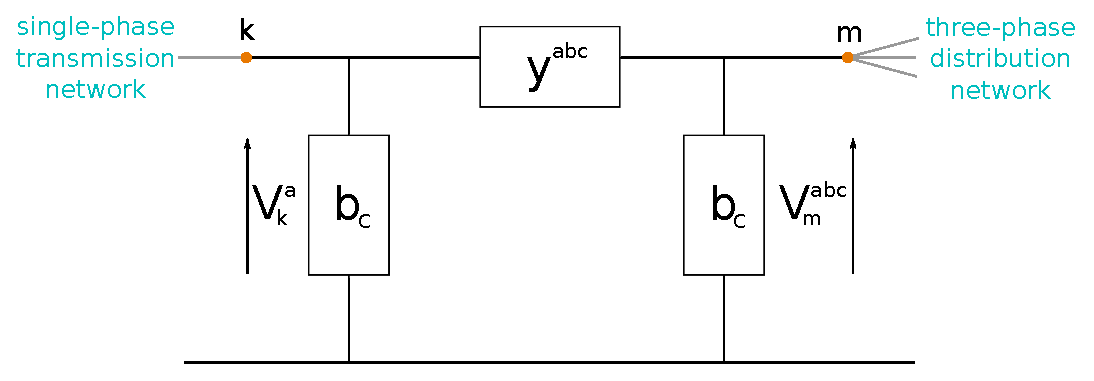
\includegraphics[width=0.8\textwidth]{Images/substationtransformer.eps}
    \caption{The original substation replaced by two buses k and m which are connected by a transformer.}
    \label{fig:subtrans}
\end{figure}
\subsubsection{{The full three-phase method}}
\label{sect:f3p}
The full three-phase method is the unified method applied on homogeneous networks and a homogeneous network consists of two three-phase networks. Unbalanced distribution networks are by default modeled in three-phase, the transmission networks requires a transformation. This transformation is based on the assumption that the transmission system is balanced: we deduct the phases $b$ and $c$ from the first phase $a$ and we transform  the voltage $V_a$, the power $S_a$, and the admittance $Y_a$ of all the buses $i=1,...,N$ to their three-phase equivalents. We transform all the buses $i=1,..,N$ in the transmission system using transformer matrices:
\begin{align}
    \mathbf{T_1}=\begin{bmatrix}1 & a & a^2\end{bmatrix}^T\quad\mbox{ and}\quad \mathbf{T_2}=\begin{bmatrix}1  & 1 & 1\end{bmatrix}^T,\quad a=e^{\frac{2}{3}\pi\iota},\nonumber
    \end{align} 
    and identity matrix $\mathbf{I}_{3\times 3}$. 
This results into the following:
\begin{align}
 \mathbf{T_1}\left[V_a\right]_i &= \begin{bmatrix} V_a & V_b & V_c\end{bmatrix}_i^T ,  \label{eq:f3pV}\\%
\mathbf{T_2}\begin{bmatrix}S_a\end{bmatrix}_i&=\begin{bmatrix} S_a & S_b & S_c\end{bmatrix}_i^T   , \label{eq:f3pS} \\%
  \begin{bmatrix}
             {Y^{a}_{11}}\otimes \mathbf{I}_{3\times 3} &  {Y^{a}_{12}}\otimes \mathbf{I}_{3\times 3} \\
               {Y^{a}_{21}}\otimes \mathbf{I}_{3\times 3} &  {Y^{a}_{22}\otimes \mathbf{I}_{3\times 3}}
              \end{bmatrix}_{ij}
&=
     \kbordermatrix{ & 3 & 3 \\
             3 & {\mathbf{Y}^{abc}_{11}} &  {\mathbf{Y}^{abc}_{12}} \\[1.5ex]
              3 &  {\mathbf{Y}^{abc}_{21}} &   {\mathbf{Y}^{abc}_{22}}
              }_{ij}.\label{eq:f3pY}%
 \end{align}


\subsubsection{{The interconnected method}}
\label{sect:ic}
The interconnected method is the unified method applied to hybrid networks. A hybrid network consists of a single-phase transmission part and a three-phase distribution part. The transformer in between load bus $k$ of the transmission network and the generator bus $m$ of the distribution network connects the information between the two networks. It couples the single-phase quantities at the transmission side to the three-phase quantities at distribution side by transforming the nodal admittance matrix $\mathbf{Y}_{km}$. We use three transformer matrices  \begin{equation}
    \mathbf{T_1}, \quad \mathbf{T_3}  = \frac{1}{3}[1\ a\ a^2],\quad\mbox{and}\quad\mathbf{T_4}= \frac{1}{3}\left[1 \ 1 \ 1 \right],\quad a = e^{\frac{2}{3}\pi\iota},
   \label{eq:T1T2}\nonumber  %= [1\ a^2\ a]^T
\end{equation} to establish the connection of bus $k$ and $m$ via the admittance matrix $\mathbf{Y}_{km}$. This transformation is based on the assumption that the connecting bus $k$ is balanced. This means that:
\begin{align}
    \begin{bmatrix}V_a & V_b & V_c\end{bmatrix}^T_k &= \mathbf{T_1}\begin{bmatrix}V_a\end{bmatrix}_k,    \label{eq:VA+}
\\
    \begin{bmatrix}I_a\end{bmatrix}_k &= \mathbf{T_3}\begin{bmatrix}I_a & I_b & I_c\end{bmatrix}^T_k,
    \label{eq:IA+}\\
     \begin{bmatrix}S_a\end{bmatrix}_k &= \mathbf{T_4}\begin{bmatrix}S_a & S_b & S_c \end{bmatrix}^T_k.\label{eq:SA+}
\end{align}
\paragraph{Using current injections}
The NR-TCIM method uses Ohm's law directly. The relation between node $k$ and $m$ is expressed as follows:
\begin{align}
    {I}=\mathbf{Y}{V}\quad\Leftrightarrow\quad\begin{bmatrix}
     I_{k} \\
     I_m
    \end{bmatrix} = \begin{bmatrix}
     Y_{11} & Y_{12} \\
     Y_{21} & Y_{22} 
    \end{bmatrix}\begin{bmatrix}
     V_k \\
     V_m
    \end{bmatrix}{}
\end{align}
If node $k$ and $m$ we're both modeled in three-phase, we know the following:
\begin{align}
   {I}_k^{abc}&=\mathbf{Y}^{abc}_{11}{V}_k^{abc}+\mathbf{Y}_{12}^{abc}{V}_m^{abc},\label{eq:IkYV}\\
   {I}_m^{abc}&=\mathbf{Y}^{abc}_{21}{V}_k^{abc}+\mathbf{Y}_{22}^{abc}{V}_m^{abc}.\label{eq:ImYV}
\end{align}
Replacing $\mathbf{V}_k^{abc}$ by $\mathbf{T_1}\begin{bmatrix}V_a\end{bmatrix}_k  $ (equation \ref{eq:VA+}) and multiplying \eqref{eq:ImYV} with $\mathbf{T_3}$ to obtain $\begin{bmatrix}I_a\end{bmatrix}_k $ (equation \eqref{eq:IA+}) results in: 
\begin{align}
  I_k^{a} = \mathbf{T_3} \mathbf{I}_k^{abc}&=\mathbf{T_3}\mathbf{Y}^{abc}_{11}\mathbf{T_1}V_k^{a}+\mathbf{T_3}\mathbf{Y}_{12}^{abc}\mathbf{V}_m^{abc},\label{eq:IkYVT}\\
    \mathbf{I}_m^{abc}&=\mathbf{Y}^{abc}_{21}\mathbf{T_1}V_k^{a}+\mathbf{Y}_{22}^{abc}{V}_m^{abc}.\label{eq:ImYVT}
\end{align}
From \eqref{eq:IkYVT} and \eqref{eq:ImYVT} we see that our new nodal admittance matrix becomes: 
\renewcommand{\kbldelim}{[}% Left delimiter
\renewcommand{\kbrdelim}{]}% Right delimiter
\begin{align}\mathbf{Y}_{km} =
\kbordermatrix{
& 1 & 3 \\
   1 &  {\mathbf{T_3} [\mathbf{Y^{abc}}_{11}] \mathbf{T_1}} & {\mathbf{T_3} [\mathbf{Y}^{abc}_{12}]}  \\
3 & [\mathbf{Y}^{abc}_{21}]{\mathbf{T_1} } & {\mathbf{Y}^{abc}_{22}} 
  }_{km}
\end{align}
\paragraph{Using power injections}
The NR-power methods uses power injections. The relation between node $k$ and $m$ is expressed as follows: 
\begin{align}
   {S}={V}{I^*}\quad\Leftrightarrow\quad\begin{bmatrix}
     S_{k} \\
     S_m
    \end{bmatrix} = \begin{bmatrix}
     V_k \\
     V_m
    \end{bmatrix}\begin{bmatrix}
    I_k \\
     I_m
    \end{bmatrix}^*
    \end{align}
In the same manner as current injections, we can write this relation in three-phase: 
\begin{align}
   {S}_k^{abc}&={V}_k^{abc}{I}_k^{abc*}+{V}_k^{abc}{I}_m^{abc*},\label{eq:SkYV}\\
   {S}_m^{abc}&={V}_m^{abc}{I}_k^{abc*}+{V}_m^{abc}{I}_m^{abc*}.\label{eq:SmYV}
\end{align}
Multiplying the first line from the left by $\mathbf{T_4}$, replacing $V_k^{abc}$ and $I_k^{abc}$ using \eqref{eq:VA+} and \eqref{eq:IA+}, and substituting $I^* = (\mathbf{Y}V)^*$ we obtain:
\begin{align}
    S_k^a = \mathbf{T_4} S^{abc}_k &= \mathbf{T_4}\mbox{diag}(\mathbf{T_1}V_k^a)\cdot \mathbf{Y}_{11}\mathbf{T_1}V_k^a + \mathbf{T_4}\mbox{diag}(\mathbf{T_1}V_k^a)\cdot \mathbf{Y}_{12}V_m^{abc}, \label{eq:STIChybk}\\ 
        S^{abc}_m &=V_m^{abc} \mathbf{Y}_{21}\mathbf{T_1}V_k^a + V_m^{abc} \mathbf{Y}_{22}V_m^{abc}. \label{eq:STIChybm}
\end{align}
We can rewrite the first part of the rhs of \eqref{eq:STIChybk} as:
\begin{align}
    \mathbf{T_4}\mbox{diag}(\mathbf{T_1}V_k^a) &= \mathbf{T_4}\mbox{diag}(\mathbf{T_1})\mbox{diag}(V_k^a) \\
    &= \frac{1}{3}\begin{bmatrix} 1 & 1 & 1 \end{bmatrix}\begin{bmatrix} 1 &0 &0 \\ 
   0 & a^2 &0 \\ 
    0& 0& a \end{bmatrix}\mbox{diag}(V_k^a) \\
    &=\underbrace{\frac{1}{3} \begin{bmatrix}1 & a^2 & a \end{bmatrix}}_{\mathbf{T_5}}\mbox{diag}(V_k^a) \\
    &\Leftrightarrow \mbox{diag}(V_k^a) \mathbf{T_5}.\label{eq:VkT6}
\end{align}
Equations \eqref{eq:STIChybk}, \eqref{eq:STIChybm}, and \eqref{eq:VkT6} results in a new admittance matrix $\mathbf{Y}_{km}$: 
\begin{align}\mathbf{Y}_{km} =
\kbordermatrix{
& 1 & 3 \\
   1 &  {\mathbf{T_5} [\mathbf{Y^{abc}}_{11}] \mathbf{T_1}} & {\mathbf{T_5} [\mathbf{Y}^{abc}_{12}]}  \\
3 & [\mathbf{Y}^{abc}_{21}]{\mathbf{T_1} } & {\mathbf{Y}^{abc}_{22}} 
  }_{km}
\end{align}
\subsection{Master-Slave splitting methods}
In contrast to the unified methods, the MSS-methods keeps two separate domains, the transmission and distribution network (or the master and the slave), and introduces an extra iterative scheme between the domains. The two domains have one overlapping bus: the substation. In the unified methods, the substation is converted to two buses connected by an extra transformer. The MSS-methods keeps the substation as one bus, which they call the boundary bus $B$. As the two domains are solved separately, the boundary bus becomes the slack bus for the distribution system and a load bus for the transmission system. In one MSS-iteration, we solve the slave, injects the solution of the boundary bus into the master, and then solve the master. This iterative process continues until the difference between the boundary bus of the slave and the master is smaller than a certain tolerance value $\epsilon$.\todo{define $\epsilon$} As the boundary bus is the slack bus of the slave, it requires the voltage $V_B$ as known information. In the first iteration, we initialize the voltage as $V_B=1.0$ pu. In the following iterations, we take the voltage from the output of the master. The boundary bus is a load bus for the master and thus requires the complex power as known. We use the output from the slave $S_B$ as input for the master. Algorithm \ref{alg:mss} shows how the iterative scheme of the MSS-method works.     
\begin{algorithm}
    \caption{General algorithmic approach of the Master-Slave splitting method}
        \label{alg:mss}
\begin{algorithmic}[1]
        \State Set iteration counter $\nu=0$. Initialize the voltage $V_B^0$ of the Slave.
        \State Solve the slave system. Output: $S_B^{\nu+1}$.
        \State Inject $S_B^{\nu+1}$ into the Master.
        \State Solve the Master. Output: $V_B^{\nu+1}$.
        \State Is $|V_B^{\nu+1}-V_B^{\nu}|_1 >  \epsilon $ ?  Repeat step 2 till 5.
    \end{algorithmic}
\end{algorithm}
As the MSS-method solves the master and slave separately, it allows for using different algorithms per domain. In this way, we choose to solve the slave with the advantageous NR-TCIM method and the master with the NR-power method.     \newline\newline
The MSS-method can be applied to homogeneous networks and to hybrid networks. The first one requiring a transformation of the entire master domain, the latter requiring a transformation of the boundary bus only. 
\subsubsection{{The MSS-homogeneous method}}
The MSS-method applied to homogeneous networks requires a transformation of the single-phase transmission system. The balanced transmission system is transformed in the same was as in the F3P-method. The voltage, power, and admittance of all the buses $i=1,..,N$ are transformed to three-phase equivalents. This idea is summarized in equations \eqref{eq:f3pV} - \eqref{eq:f3pY} of section \ref{sect:f3p}. Note that there is no connecting transformer between the transmission and distribution system: The output $S_B$ of the slave can be directly injected into the master. 

\subsubsection{{The MSS-hybrid method}}
The MSS-method applied to hybrid systems keeps the transmission system in single-phase. Only a transformation of the boundary bus is then required. \newline
As we first solve the slave, we receive the complex power $S_B$ as three-phase output, which we have to transform to a single-phase quantity. Once we have solved the master, we have to transform the single-phase output of the voltage $V_B$ of the master. Here again, we assume that the boundary bus $B$ is balanced. Balanced three-phase power in pu is related to single-phase power in \eqref{eq:SA+}:
\begin{align}
    [S_a] = \mathbf{T_4}\begin{bmatrix}S_a & S_b & S_c \end{bmatrix}^T.
\label{eq:MSShS}\end{align}
We transform the complex power of the boundary bus $[S_{abc}]_B$ to $[S_a]_B$ using equation \eqref{eq:MSShS}. \newline 
The voltage of the boundary bus has the same relation as in \eqref{eq:VA+}: 
\begin{align}
    \begin{bmatrix}V_a & V_b & V_c\end{bmatrix}^T_B &= \mathbf{T_1}\begin{bmatrix}V_a\end{bmatrix}_B,\quad 
     \mathbf{T_1} = [1\ a^2\ a]^T\quad\mbox{and}\quad a = e^{\frac{2}{3}\pi\iota}.\label{eq:MSShV}
    \end{align}
The MSS-methods do not require a transformation of the nodal admittance matrix. We transform the necessary boundary parameters directly. At every MSS-iteration, we make transformation \eqref{eq:MSShS} and \eqref{eq:MSShV} after step 2 and step 4 of algorithm \ref{alg:mss}, respectively. 

\subsubsection{The Master-Slave iterative schemes}
Two iterative schemes of the Master-Slave splitting are defined \cite{Sun2011}. The first is the Convergence Alternating Iterative (CAI) scheme and the other is the Multistep Alternating Iterative (MAI) scheme. In the CAI-scheme, we define an explicit convergence condition for the slave and for the master. The slave is solved with NR-TCIM, for which we define a tolerance value $\epsilon_D$\todo{Give $\epsilon$}. Once this system has converged, we inject its boundary output into the master. We solve the master using NR-power, for which we also define a (not necessarily) different tolerance value $\epsilon_T$. Once the master has converged, we inject its boundary output into the slave. The integrated network is converged once we have met the convergence condition of the MSS-algorithm. \\
In the MAI-scheme, we define a maximum number of iterations per separate system, ie: $I_{max,D}$ and $I_{max,T}$. We inject the output of one system into the other as soon this maximum number of iterations has been reached. The convergence of the integrated network is still based on the convergence condition of the MSS-algorithm. 
\paragraph{Speeding up the CAI-scheme} \label{par:caischeme}
At every MSS iteration, we solve the separated domains on its own. To solve this separated system, we need to initialize the voltages in order to have an initial guess to start Newton-Raphson. In the current suggested schemes, we initialize all the buses, except the boundary bus $B$, to $V=1.0$ pu.\todo{Clarify the coming phrase} We can reduce the number of required iterations for the separate systems if we initialize the voltages to its last obtained solution in the previous MSS-iteration, ie $V^{\nu+1}_0=V^{\nu}_{I,D}$. This will probably be beneficial for the CAI-scheme, where a separated domain requires a couple of iterations before it is converged.  






\newpage 
\section{Numerical assessment}
All previous mentioned methods are implemented into the Matpower\footnote{MATPOWER is a package of free, open-source Matlab-language M-files for solving steady-state power system simulation and optimization problems \cite{Zimmerman2011}} library. Matpower consists of several transmission network test cases. The resources page of IEEE Power \& Energy Society  contains several distribution network test cases which are all explained in \cite{Schneider2018}. These test cases contain the necessary input to solve power flow problems. We created integrated test test cases from the existing transmission and distribution test cases. We used the IEEE 9-bus, 118-bus, and 3120-bus data as transmission network test cases and the IEEE 13-bus and 37-bus data as distribution test cases. The distribution test cases represent the unbalanced characteristics of the network. We modified the 13-bus distribution network to a 10-bus network by deleting the buses connected to the regulator. We changed the loading of the 37-bus network by shifting 20\% of the loads of phase b equally to phase a and c, just like the original authors \cite{Taranto2008}.
We connected two networks to each other creating the following integrated test cases: 
\begin{itemize}
    \item Test case 1: T9-D13
    \item Test case 2: T9-D37
    \item Test case 3: T118-D37
    \item Test case 4: T3120-D37
    \item Test case 5: T9-2D13 (2 13-bus distribution networks) 
    \item Test case 6: T9-3D13 (3 13-bus distribution networks) 
\end{itemize}
\paragraph{Connection bus}
We selected a random load bus in the transmission network to become the connection bus in the integrated network. We choose bus $7$ in the 9-bus network, we choose bus $118$ in the 118-bus network, and we choose bus $3003$ in the 3120-bus network. This could have been any load bus of the original network. The original reference bus of the distribution network becomes the connection bus in the integrated network. \\
The unified methods puts a transformer between the connection buses. This transformer has the same line admittance as the first distribution cable. The left hand side of the transformer is the transmission connection bus, now having zero load. The right hand side is the distribution connection bus. This is the former reference bus and must be changed to a load bus having the load as the original transmission connection bus \cite{Taranto2008}. The splitting methods do not put a transformer between the networks. They only change the original transmission load bus to a bus having zero load.   \newline \newline
Test case 5 and 6 have multiple distribution networks connected. These networks are connected to the last 2 and 3 load buses of the transmission networks, where each of the original load bus is changed to a zero load bus. 
\subsection{Results}
We are going to compare the above-mentioned methods on accuracy, speed, and convergence to give an insight into which method is favorable to solve integrated networks. 
\subsubsection{Accuracy} 
To check the accuracy of the methods, we compare the voltage output of the integrated methods with the output of the separated methods. We solve the transmission network separately using NR-power and we solve the distribution network separately using NR-TCIM. The distribution domain in the integrated network has no reference bus anymore. In order to compare the voltage profile of this part, we scale the values accordingly. \\
We know that the voltage is given by: \begin{equation}
V_p=|V|_p\exp{(\iota\delta_{V_p}-\phi)},\quad p\in\{a,b,c\},
\end{equation}
where $|V|$ and $\delta$ are set to $|V|=1.0$ pu and $\delta=0$ at the reference bus. We can compare the voltage of the distribution domain to the voltage of the separated domain after scaling. We divide the voltage magnitude of the distribution domain, buses $i=1,...,D_N$ by the voltage magnitude of the distribution connection bus: 
\begin{equation}
|V|_{i,{D_{new}}} = \frac{|V|_{i,{D_{uns}}}}{|V|_{ref,{D_{uns}}}},\quad i=1,..,D_N.
\label{eq:ViDnew}
\end{equation}
The voltage angle represents the phase-shift in relation to the reference bus. In order to compare the integrated output of the voltage angle with the separated output, we subtract the phase-angle of the former reference bus of all the buses of the distribution domain: 
\begin{equation}
\delta_{i,{D_{new}}} ={\delta_{i,{D_{uns}}}}-{\delta_{ref,{D_{uns}}}},\quad i=1,..,D_N.
\label{eq:dViDnew}
\end{equation}
Note that we need to apply \eqref{eq:ViDnew} and \eqref{eq:dViDnew} to all the three phases separately. \newline\newline
We compare the voltage magnitudes and angles of the integrated network, including the scaled distribution domain, with the magnitudes angles of the separate domains. We take the infinity norm of the relative difference between the voltages: spee
\begin{equation}
\mbox{rel. error of } |V|_p = \left|\frac{|V|^*_p - |V|^o_p}{|V|^o_p}\right|_\infty,\quad p\in\{a,b,c\},
\label{eq:norm|V|}
\end{equation}
where the asterisk $*$ marks the outcome of separated networks, and the superscript $o$ the output of separated networks (original). We do this in a similar manner for the voltage angle: 
\begin{equation}
\mbox{rel. error of } \delta_p = \left|\frac{\delta^*_p - \delta^o_p}{\delta^o_p}\right|_\infty,\quad p\in\{a,b,c\},
\label{eq:normdelta}
\end{equation}
We have given the relative errors of the voltage magnitude and angle of the three phases for all the test cases in table \ref{tab:relerror}. 

\begin{table}[h]
\renewcommand{\arraystretch}{1.3}
\centering
\caption{Relative error of the voltage magnitude and angle of the three phases for all the integration methods. }\label{tab:relerror}
\begin{adjustbox}{width=1\textwidth} %, angle=90}
\small
\begin{tabular}{ccccccccc}
\toprule
{} && \multicolumn{7}{c}{Full three-phase}   \\
\cmidrule{3-9}
{} && \multicolumn{3}{c}{$|V|$} && \multicolumn{3}{c}{$\delta$}  \\
\cmidrule{3-5}\cmidrule{7-9}
 test case &&        a &        b &       c &&        a &       b &        c \\
\midrule
T9-D13    &&  3.854e-04 &  6.851e-04 &  2.000e-04 &&  -6.119e-03 &  -5.376e-03 &  -6.475e-03 \\
T9-D37    &&  4.000e-04 &  5.153e-04 &  4.100e-04 &&   3.769e-01 &  -1.230e-02 &   1.529e-01 \\
T118-D37  &&  9.791e-05 &  6.000e-05 &  7.000e-05 &&   3.979e-01 &   3.600e-01 &   4.237e-01 \\
T3120-D37 &&  2.409e-04 &  7.524e-04 &  1.293e-04 &&   2.271e+00 &   2.121e-01 &   2.495e-01 \\
\bottomrule
\end{tabular}
\end{adjustbox}
%N2I1

\begin{adjustbox}{width=1\textwidth} %, angle=90}
\small
\begin{tabular}{ccccccccc}
\toprule
{test case} && \multicolumn{7}{c}{MSS-homo-CAI}   \\
%\cmidrule{3-9}
%{} && \multicolumn{3}{c}{$|V|$} && \multicolumn{3}{c}{$\delta$}  \\
%\cmidrule{3-5}\cmidrule{7-9}
 %test-case &&        a &        b &       c &&        a &       b &        c \\
\midrule
T9-D13       &&  2.934e-04 &  7.982e-04 &  2.874e-04 &&  4.794e-02 &  4.246e-02 &  5.097e-02 \\
T9-D37       &&  1.916e-04 &  5.394e-04 &  1.916e-04 &&  2.271e+00 &  1.571e-02 &  3.297e-02 \\
T118-D37     &&  8.984e-03 &  8.911e-03 &  9.005e-03 &&  4.501e-01 &  4.468e-01 &  4.524e-01 \\
T3120-D37    &&  2.440e-04 &  7.296e-04 &  1.303e-04 &&  3.434e-01 &  1.951e-02 &  4.082e-02 \\
%MaxT9-D13    &&         14 &         16 &          6 &&          3 &          3 &          3 \\
%MaxT9-D37    &&          6 &         41 &          6 &&         23 &          3 &          3 \\
%MaxT118-D37  &&        117 &        117 &        117 &&         92 &         92 &         92 \\
%MaxT3120-D37 &&       3137 &       3152 &       3126 &&       3133 &       2017 &       2017 \\
\bottomrule
\end{tabular}
\end{adjustbox}
%N2I2
\begin{adjustbox}{width=1\textwidth} %, angle=90}
\small
\begin{tabular}{ccccccccc}
\toprule
{test case} && \multicolumn{7}{c}{MSS-homo-MAI, 2 iterations per subdomain}   \\
%\cmidrule{3-9}
%{} && \multicolumn{3}{c}{$|V|$} && \multicolumn{3}{c}{$\delta$}  \\
%\cmidrule{3-5}\cmidrule{7-9}
% test-case &&        a &        b &       c &&        a &       b &        c \\
\midrule
T9-D13       &&  5.749e-04 &  7.037e-04 &  5.749e-04 &&  6.702e-02 &  1.231e+00 &  1.261e+00 \\
T9-D37       &&  4.364e-04 &  4.796e-04 &  3.958e-04 &&  2.587e+01 &  2.724e-02 &  1.011e+01 \\
T118-D37     &&  2.017e-01 &  2.017e-01 &  2.017e-01 &&  1.993e+01 &  1.993e+01 &  1.993e+01 \\
T3120-D37    &&  1.048e-01 &  1.048e-01 &  1.048e-01 &&  4.504e+02 &  1.535e+01 &  8.085e+01 \\
%MaxT9-D13    &&          6 &         16 &          6 &&          8 &         11 &         11 \\
%MaxT9-D37    &&          8 &         19 &          8 &&         22 &          8 &         31 \\
%MaxT118-D37  &&         82 &         82 &         82 &&         92 &         92 &         92 \\
%MaxT3120-D37 &&         32 &         32 &         32 &&       3134 &       2009 &       3128 \\
\bottomrule
\end{tabular}
\end{adjustbox}
%IC
%\label{}\hspace{2cm}%\caption{Relative error of the voltage magnitude and angle of the three phases obtained using the interconnected method. }
\begin{adjustbox}{width=1\textwidth} %, angle=90}
\small
\begin{tabular}{ccccccccc}
\toprule
{test case} && \multicolumn{7}{c}{Interconnected}   \\
%\cmidrule{3-9}
%{} && \multicolumn{3}{c}{$|V|$} && \multicolumn{3}{c}{$\delta$}  \\
%\cmidrule{3-5}\cmidrule{7-9}
% test-case &&        a &        b &       c &&        a &       b &        c \\
\midrule
T9-D13    &&  2.895e-04 &  6.851e-04 &  2.000e-04 &&  -6.000e-03 &  -6.000e-03 &  -6.000e-03 \\
T9-D37    &&  4.000e-04 &  5.247e-04 &  4.000e-04 &&   3.769e-01 &   3.769e-01 &   3.769e-01 \\
T118-D37  &&  9.791e-05 &  7.000e-05 &  7.000e-05 &&   3.939e-01 &   3.939e-01 &   3.939e-01 \\
T3120-D37 &&  2.409e-04 &  7.180e-04 &  1.593e-04 &&   3.434e-01 &   2.320e-01 &   2.320e-01 \\
\bottomrule
\end{tabular}
\end{adjustbox}

%N1I1
\begin{adjustbox}{width=1\textwidth} %, angle=90}
\small
\begin{tabular}{ccccccccc}
\toprule
{test case} && \multicolumn{7}{c}{MSS-hybrid-CAI}   \\
%\cmidrule{3-9}
%{} && \multicolumn{3}{c}{$|V|$} && \multicolumn{3}{c}{$\delta$}  \\
%\cmidrule{3-5}\cmidrule{7-9}
% test-case &&        a &        b &       c &&        a &       b &        c \\
\midrule
T9-D13       &&  2.934e-04 &  7.982e-04 &  2.874e-04 &&  4.712e-02 &  4.712e-02 &  4.712e-02 \\
T9-D37       &&  1.916e-04 &  5.299e-04 &  1.916e-04 &&  3.434e-01 &  2.487e-02 &  1.529e-01 \\
T118-D37     &&  8.963e-03 &  8.963e-03 &  8.963e-03 &&  4.497e-01 &  4.497e-01 &  4.497e-01 \\
T3120-D37    &&  2.440e-04 &  7.296e-04 &  1.303e-04 &&  2.271e+00 &  3.085e-02 &  1.529e-01 \\
%MaxT9-D13    &&         14 &         16 &          6 &&          3 &          3 &          3 \\
%MaxT9-D37    &&          6 &         40 &          6 &&         22 &          3 &         17 \\
%MaxT118-D37  &&        117 &        117 &        117 &&         92 &         92 &         92 \\
%MaxT3120-D37 &&       3137 &       3152 &       3126 &&       3134 &       2017 &       3128 \\
\bottomrule
\end{tabular}
\end{adjustbox}

%N1I2
\begin{adjustbox}{width=1\textwidth} %, angle=90}
\small
\begin{tabular}{ccccccccc}
\toprule
{test case} && \multicolumn{7}{c}{MSS-hybrid-MAI, 2 iterations per subdomain}   \\
%\cmidrule{3-9}
%{} && \multicolumn{3}{c}{$|V|$} && \multicolumn{3}{c}{$\delta$}  \\
%\cmidrule{3-5}\cmidrule{7-9}
% test-case &&        a &        b &       c &&        a &       b &        c \\
\midrule
T9-D13       &&  5.749e-04 &  7.037e-04 &  5.749e-04 &&  6.932e-02 &  1.295e+00 &  1.261e+00 \\
T9-D37       &&  4.262e-04 &  5.400e-04 &  4.262e-04 &&  2.721e+01 &  3.459e-02 &  1.011e+01 \\
T118-D37     &&  2.017e-01 &  2.017e-01 &  2.017e-01 &&  1.993e+01 &  1.993e+01 &  1.993e+01 \\
T3120-D37    &&  1.048e-01 &  1.048e-01 &  1.048e-01 &&  4.504e+02 &  1.536e+01 &  8.085e+01 \\
%MaxT9-D13    &&          6 &         16 &          6 &&          8 &         11 &         11 \\
%MaxT9-D37    &&          8 &         41 &          8 &&         22 &          8 &         31 \\
%MaxT118-D37  &&         82 &         82 &         82 &&         92 &         92 &         92 \\
%MaxT3120-D37 &&         32 &         32 &         32 &&       3134 &       2009 &       3128 \\
\bottomrule
\end{tabular}
\end{adjustbox}
\end{table}
\paragraph{The MAI-scheme}
Table \ref{tab:relerror} shows that all the integration methods produce accurate results, except for the MSS-homo-MAI and MSS-hybrid-MAI methods. This is caused by the number of iterations per subdomain that has been set too strict. To produce more accurate results, we increased the number of iterations per subdomain simultaneously. We started with $I_{T,max}=I_{D,max}=2$ until $I_{T,max}=I_{D,max}=6$.  Table \ref{tab:MAIschemes} shows the results. Next to the relative error, this table shows the required number of MSS iterations and how long it takes to reach convergence. We only applied these tests on test case T118-D37, as these results were least accurate. When using $4$ iterations per subdomain, the results become as accurate as the MSS-CAI methods. 
\begin{table}[h]
\renewcommand{\arraystretch}{1.3}
\centering
\caption{The relative error of the voltage of test case T118-D37, solved using the MAI-iterative scheme with increasing number of subiterations, $I_T, I_D$, applied on a homogeneous network (top) and on a hybrid network (bottom).}\label{tab:MAIschemes}
\begin{adjustbox}{width=1\textwidth} %, angle=90}
\small
\begin{tabular}{cccccccccccc}
\toprule
{} && \multicolumn{7}{c}{MSS-homo-MAI} && &  \\
\cmidrule{3-9}
{} && \multicolumn{3}{c}{$|V|$} && \multicolumn{3}{c}{$\delta$} && \\
\cmidrule{3-5}\cmidrule{7-9}
{$I_T$,$I_D$} &&        a &        b &       c &&        a &       b &        c && sec & $I_{MSS}$\\
\midrule
2 &&  2.017e-01 &  2.017e-01 &  2.017e-01 &&  1.993e+01 &  1.993e+01 &  1.993e+01 && 0.325 & 4 \\
3 &&  3.436e-02 &  3.436e-02 &  3.436e-02 &&  7.153e+00 &  7.150e+00 &  7.156e+00 && 0.368 & 5 \\
4 &&  9.069e-03 &  9.005e-03 &  9.100e-03 &&  7.426e-01 &  7.393e-01 &  7.448e-01 && 0.323 & 3\\
5 &&  8.984e-03 &  8.911e-03 &  9.005e-03 &&  4.507e-01 &  4.474e-01 &  4.530e-01 && 0.351 & 3\\
6 &&  8.984e-03 &  8.911e-03 &  9.005e-03 &&  4.501e-01 &  4.468e-01 &  4.524e-01 && 0.347 & 3\\
\bottomrule
\end{tabular}
\end{adjustbox}
%N1 
\begin{adjustbox}{width=1\textwidth} %, angle=90}
\small
\begin{tabular}{cccccccccccc}
\toprule
{} && \multicolumn{7}{c}{MSS-hybrid-MAI} && &  \\
\cmidrule{3-9}
{} && \multicolumn{3}{c}{$|V|$} && \multicolumn{3}{c}{$\delta$} && \\
\cmidrule{3-5}\cmidrule{7-9}
{$I_T$,$I_D$} &&        a &        b &       c &&        a &       b &        c && sec & $I_{MSS}$\\
\midrule
2 &&  2.017e-01 &  2.017e-01 &  2.017e-01 &&  1.993e+01 &  1.993e+01 &  1.993e+01 && 0.358 & 4 \\
3 &&  3.436e-02 &  3.436e-02 &  3.436e-02 &&  7.153e+00 &  7.153e+00 &  7.153e+00 && 0.380& 5\\
4 &&  9.058e-03 &  9.058e-03 &  9.058e-03 &&  7.422e-01 &  7.422e-01 &  7.422e-01 && 0.353& 3\\
5 &&  8.963e-03 &  8.963e-03 &  8.963e-03 &&  4.504e-01 &  4.504e-01 &  4.504e-01 && 0.354& 3 \\
6 &&  8.963e-03 &  8.963e-03 &  8.963e-03 &&  4.497e-01 &  4.497e-01 &  4.497e-01 && 0.351&3\\
\bottomrule
\end{tabular}
\end{adjustbox}

\end{table}

We plotted the voltage magnitude and angles of the MAI-schemes to show how the solution is with every increase of the maximum number of subiterations approaching its 'true' results. For comparison we plotted the separated transmission and distribution network as 'true' solution. 
\begin{figure}[!ht]
\centering
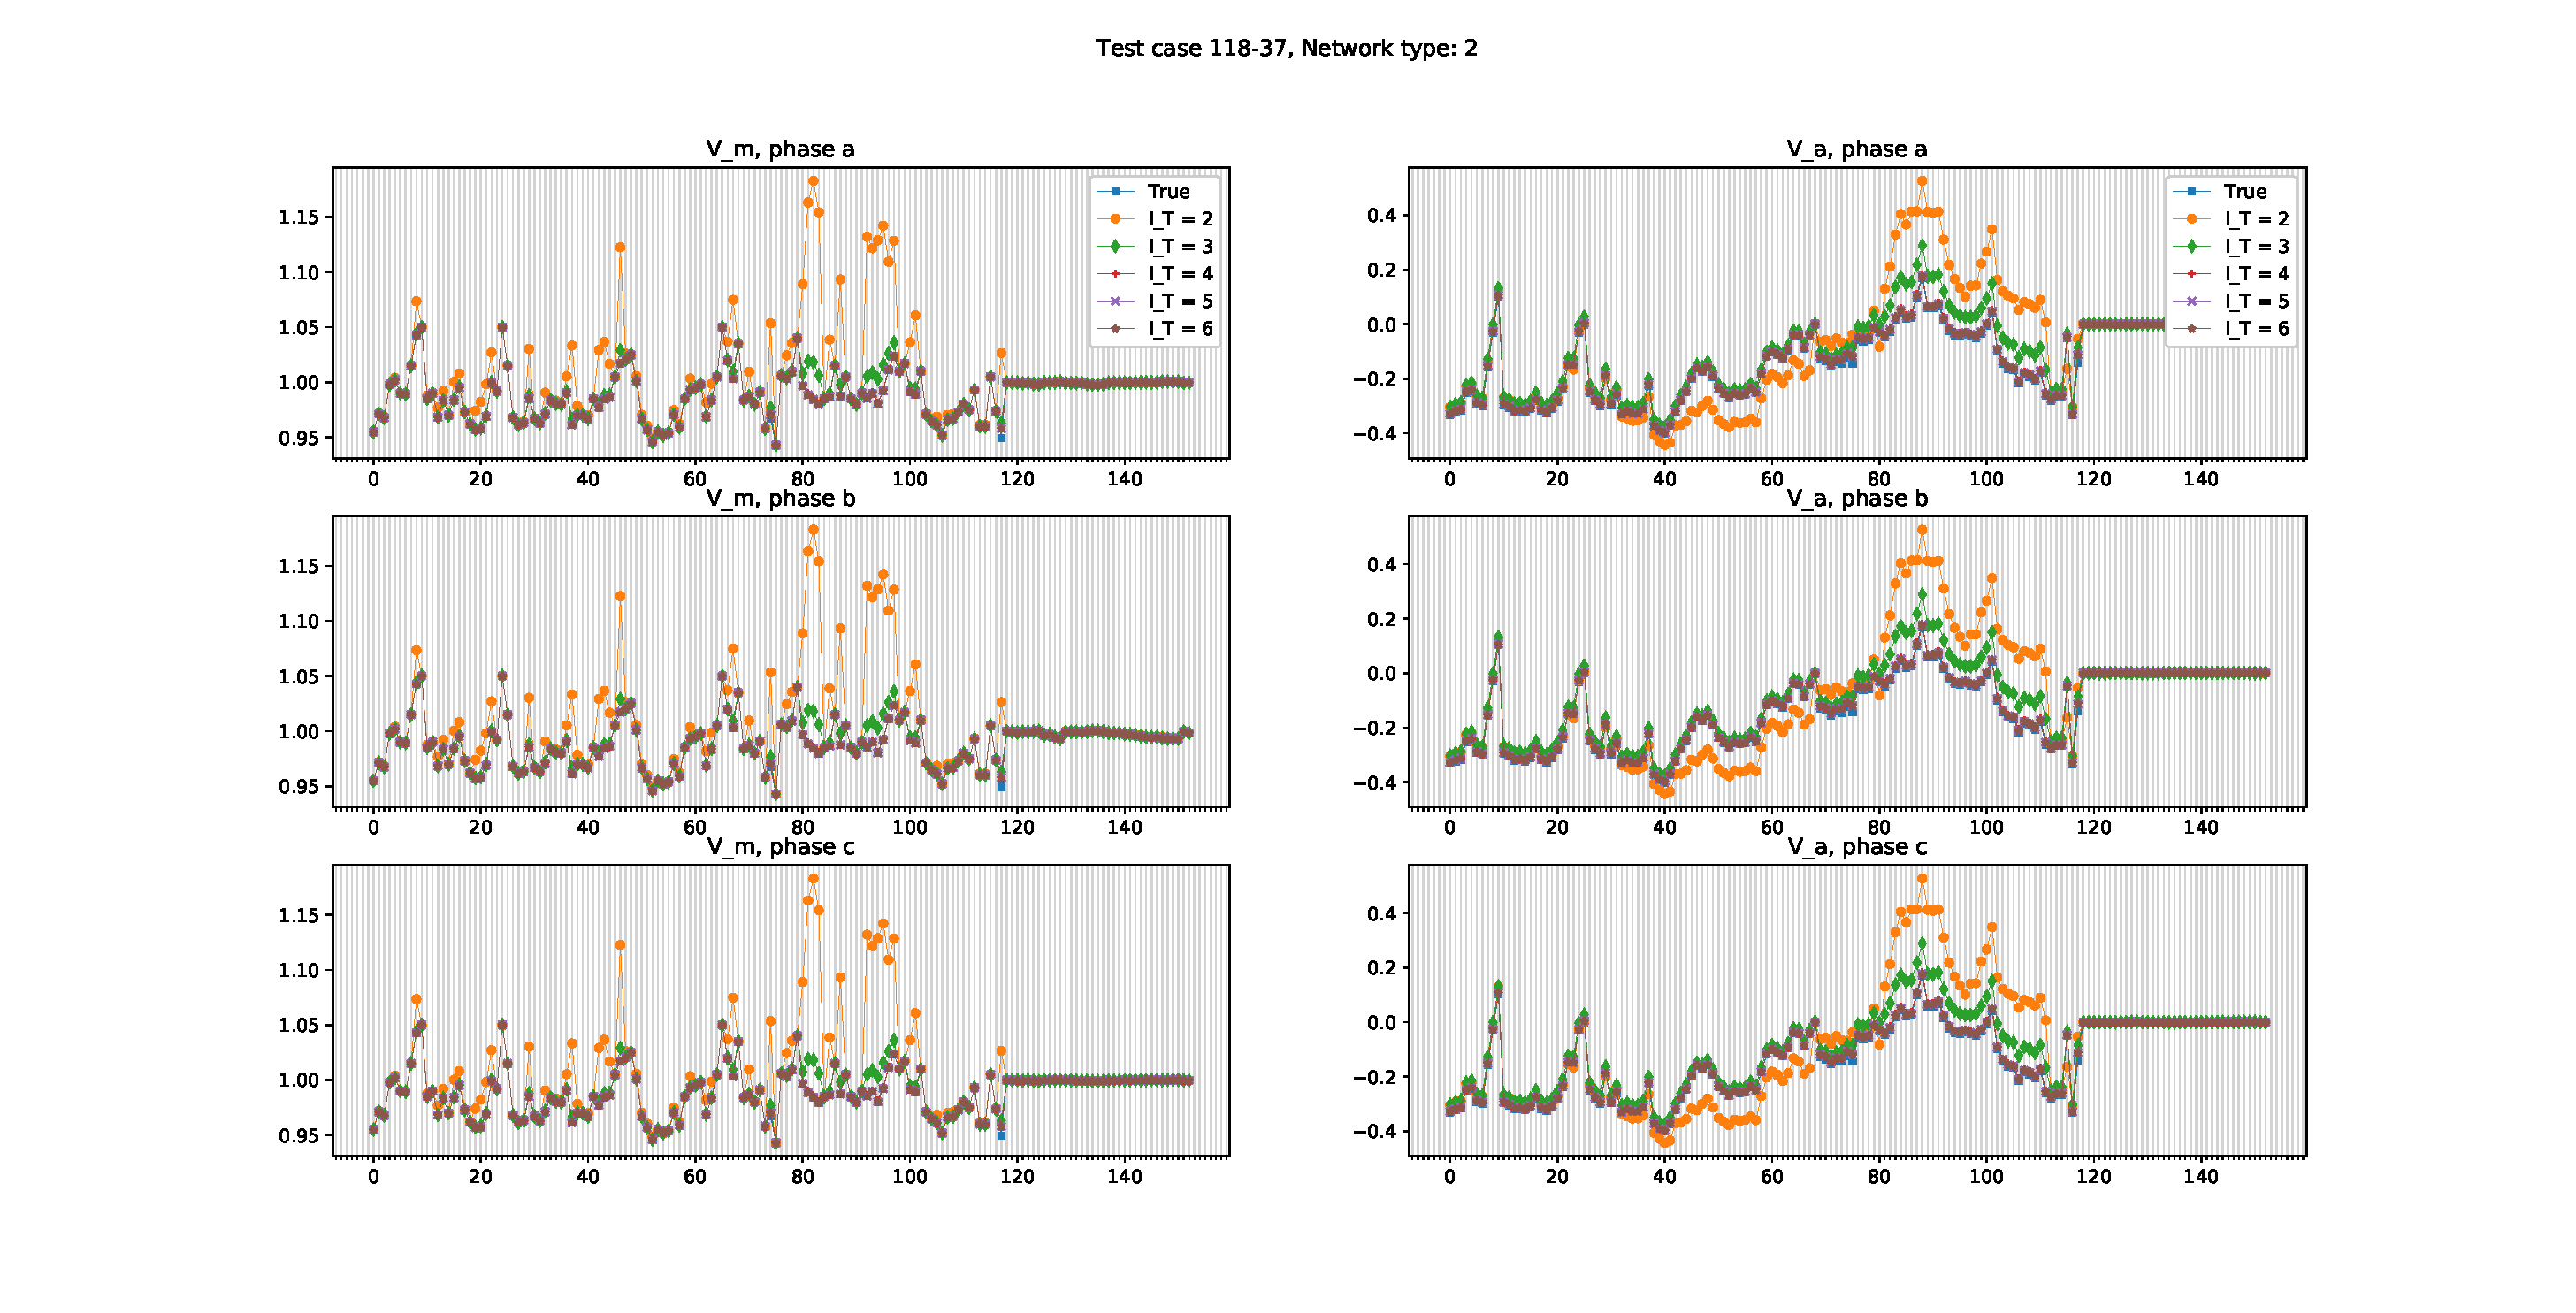
\includegraphics[width=\textwidth]{Images/MAI_N2.eps}
\caption{Voltage profile (left: magnitude, right: angle) of the MAI-schemes with increasing number of subiterations, applied on homogeneous networks}\label{fig:MAIN2}
\end{figure}
\begin{figure}[!ht]
\centering
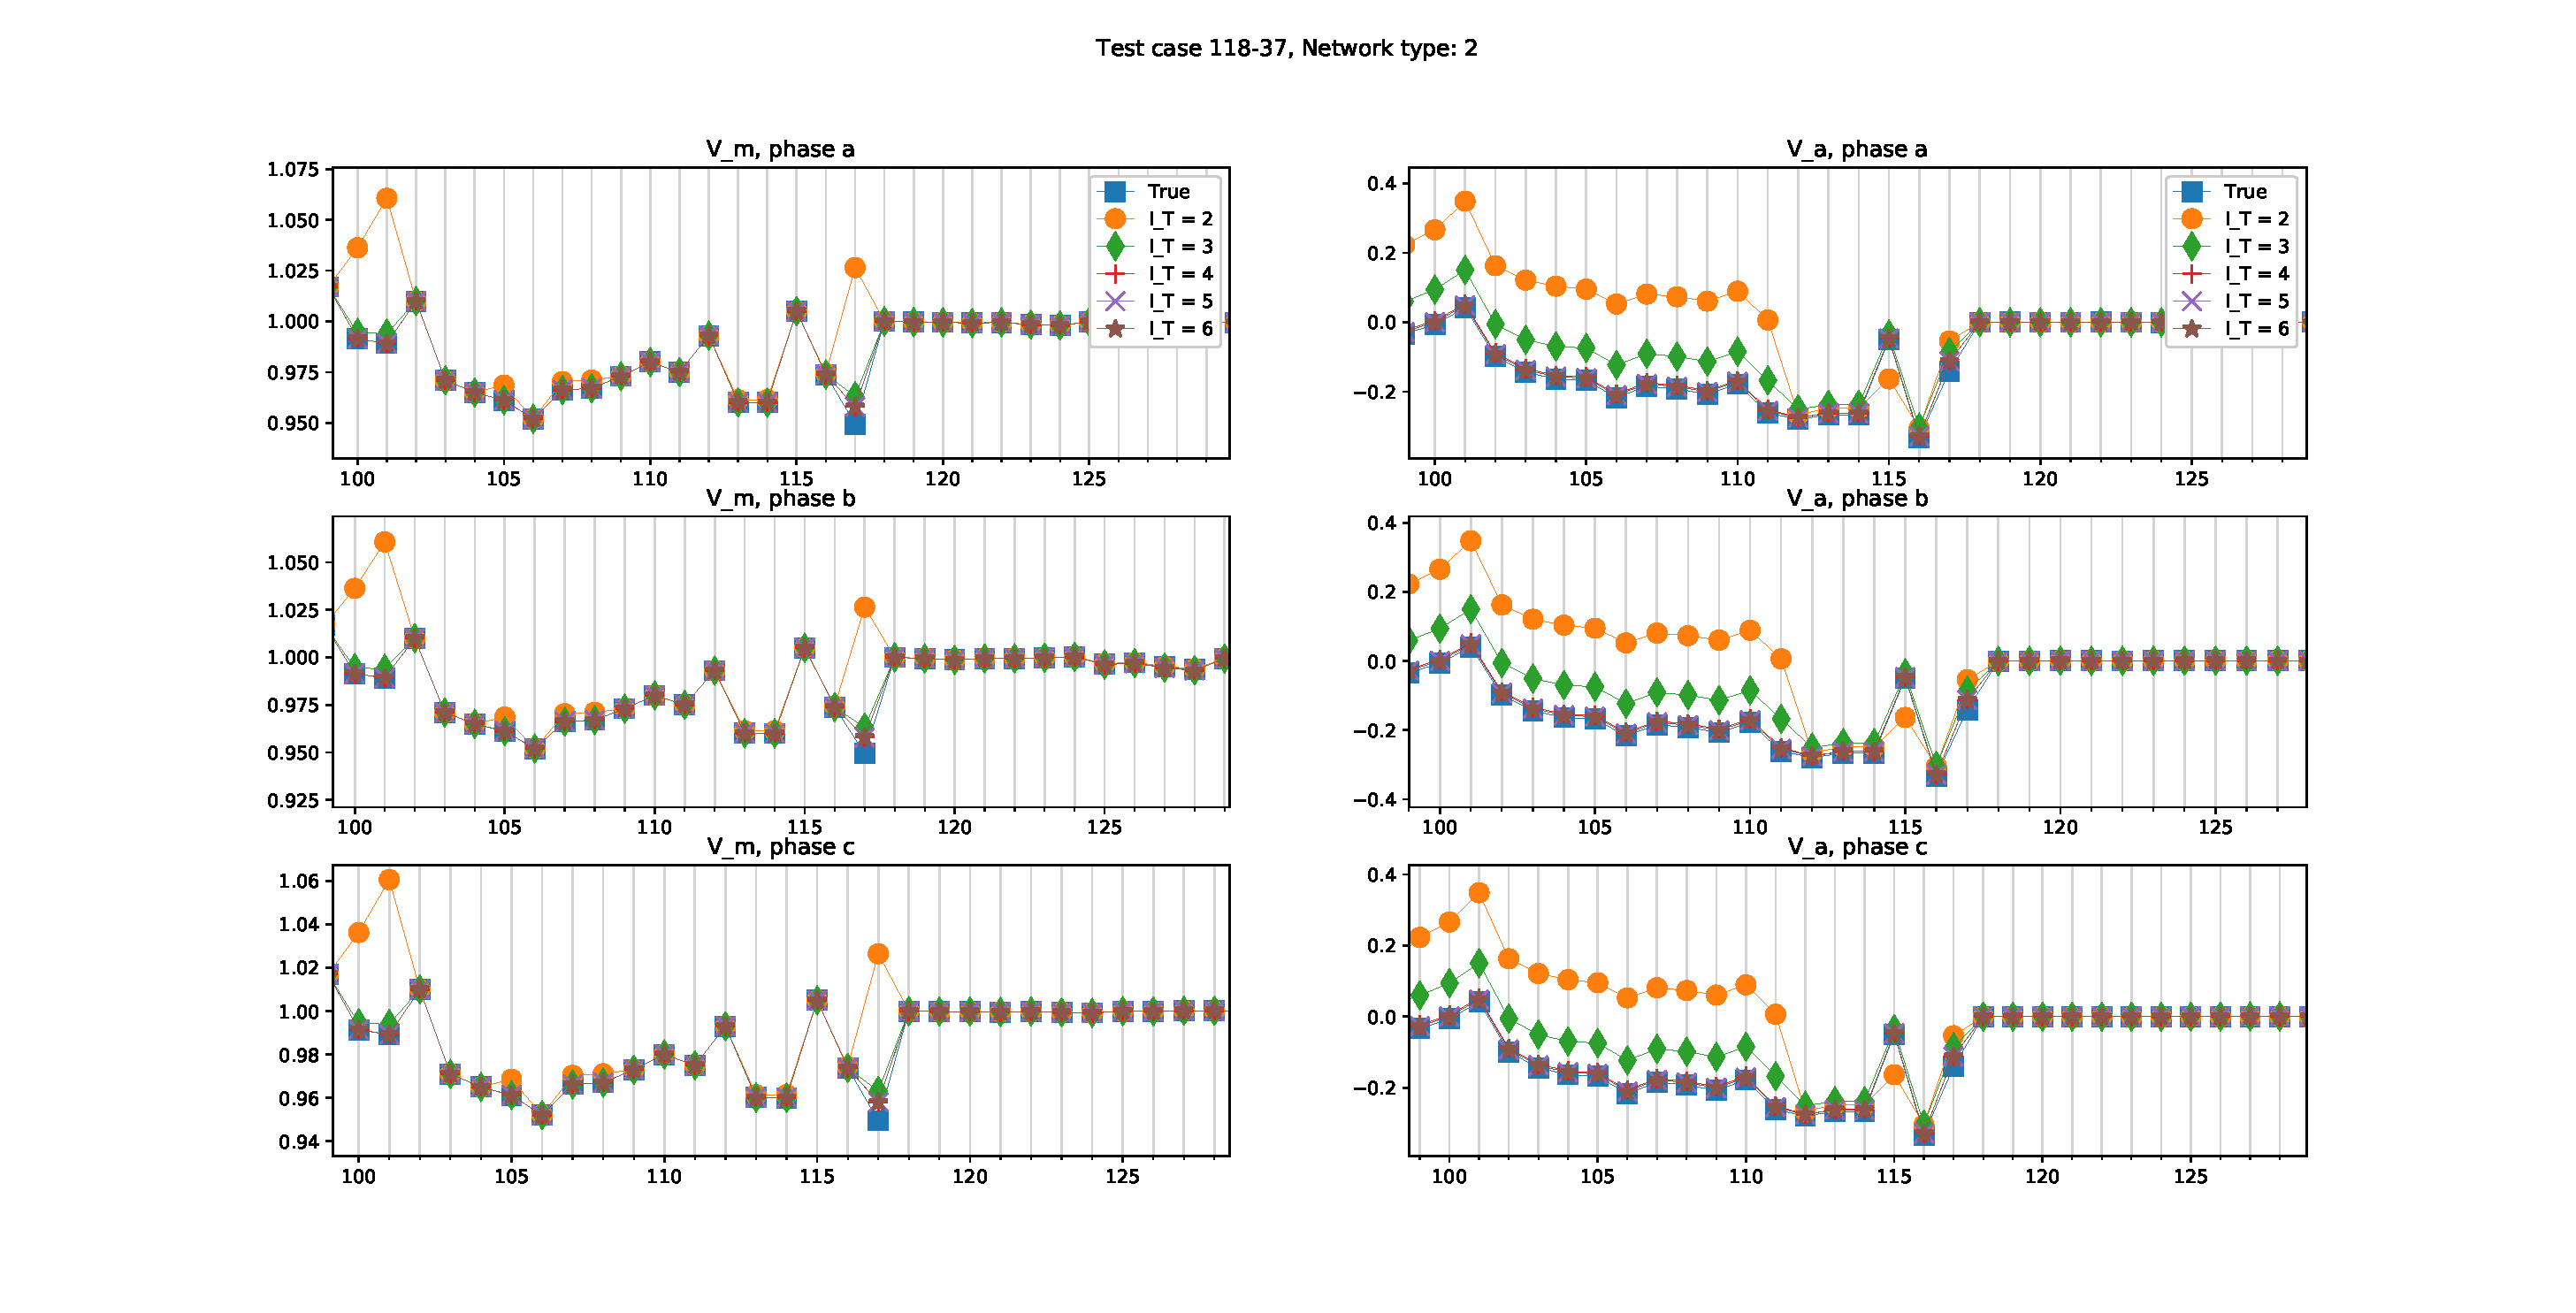
\includegraphics[width=\textwidth]{Images/Z_MAI_N2.eps}
\caption{A magnified version of the top figure of the buses surrounding the connection bus.}\label{fig:ZMAIN2}
\end{figure}
\begin{figure}[!ht]
\centering
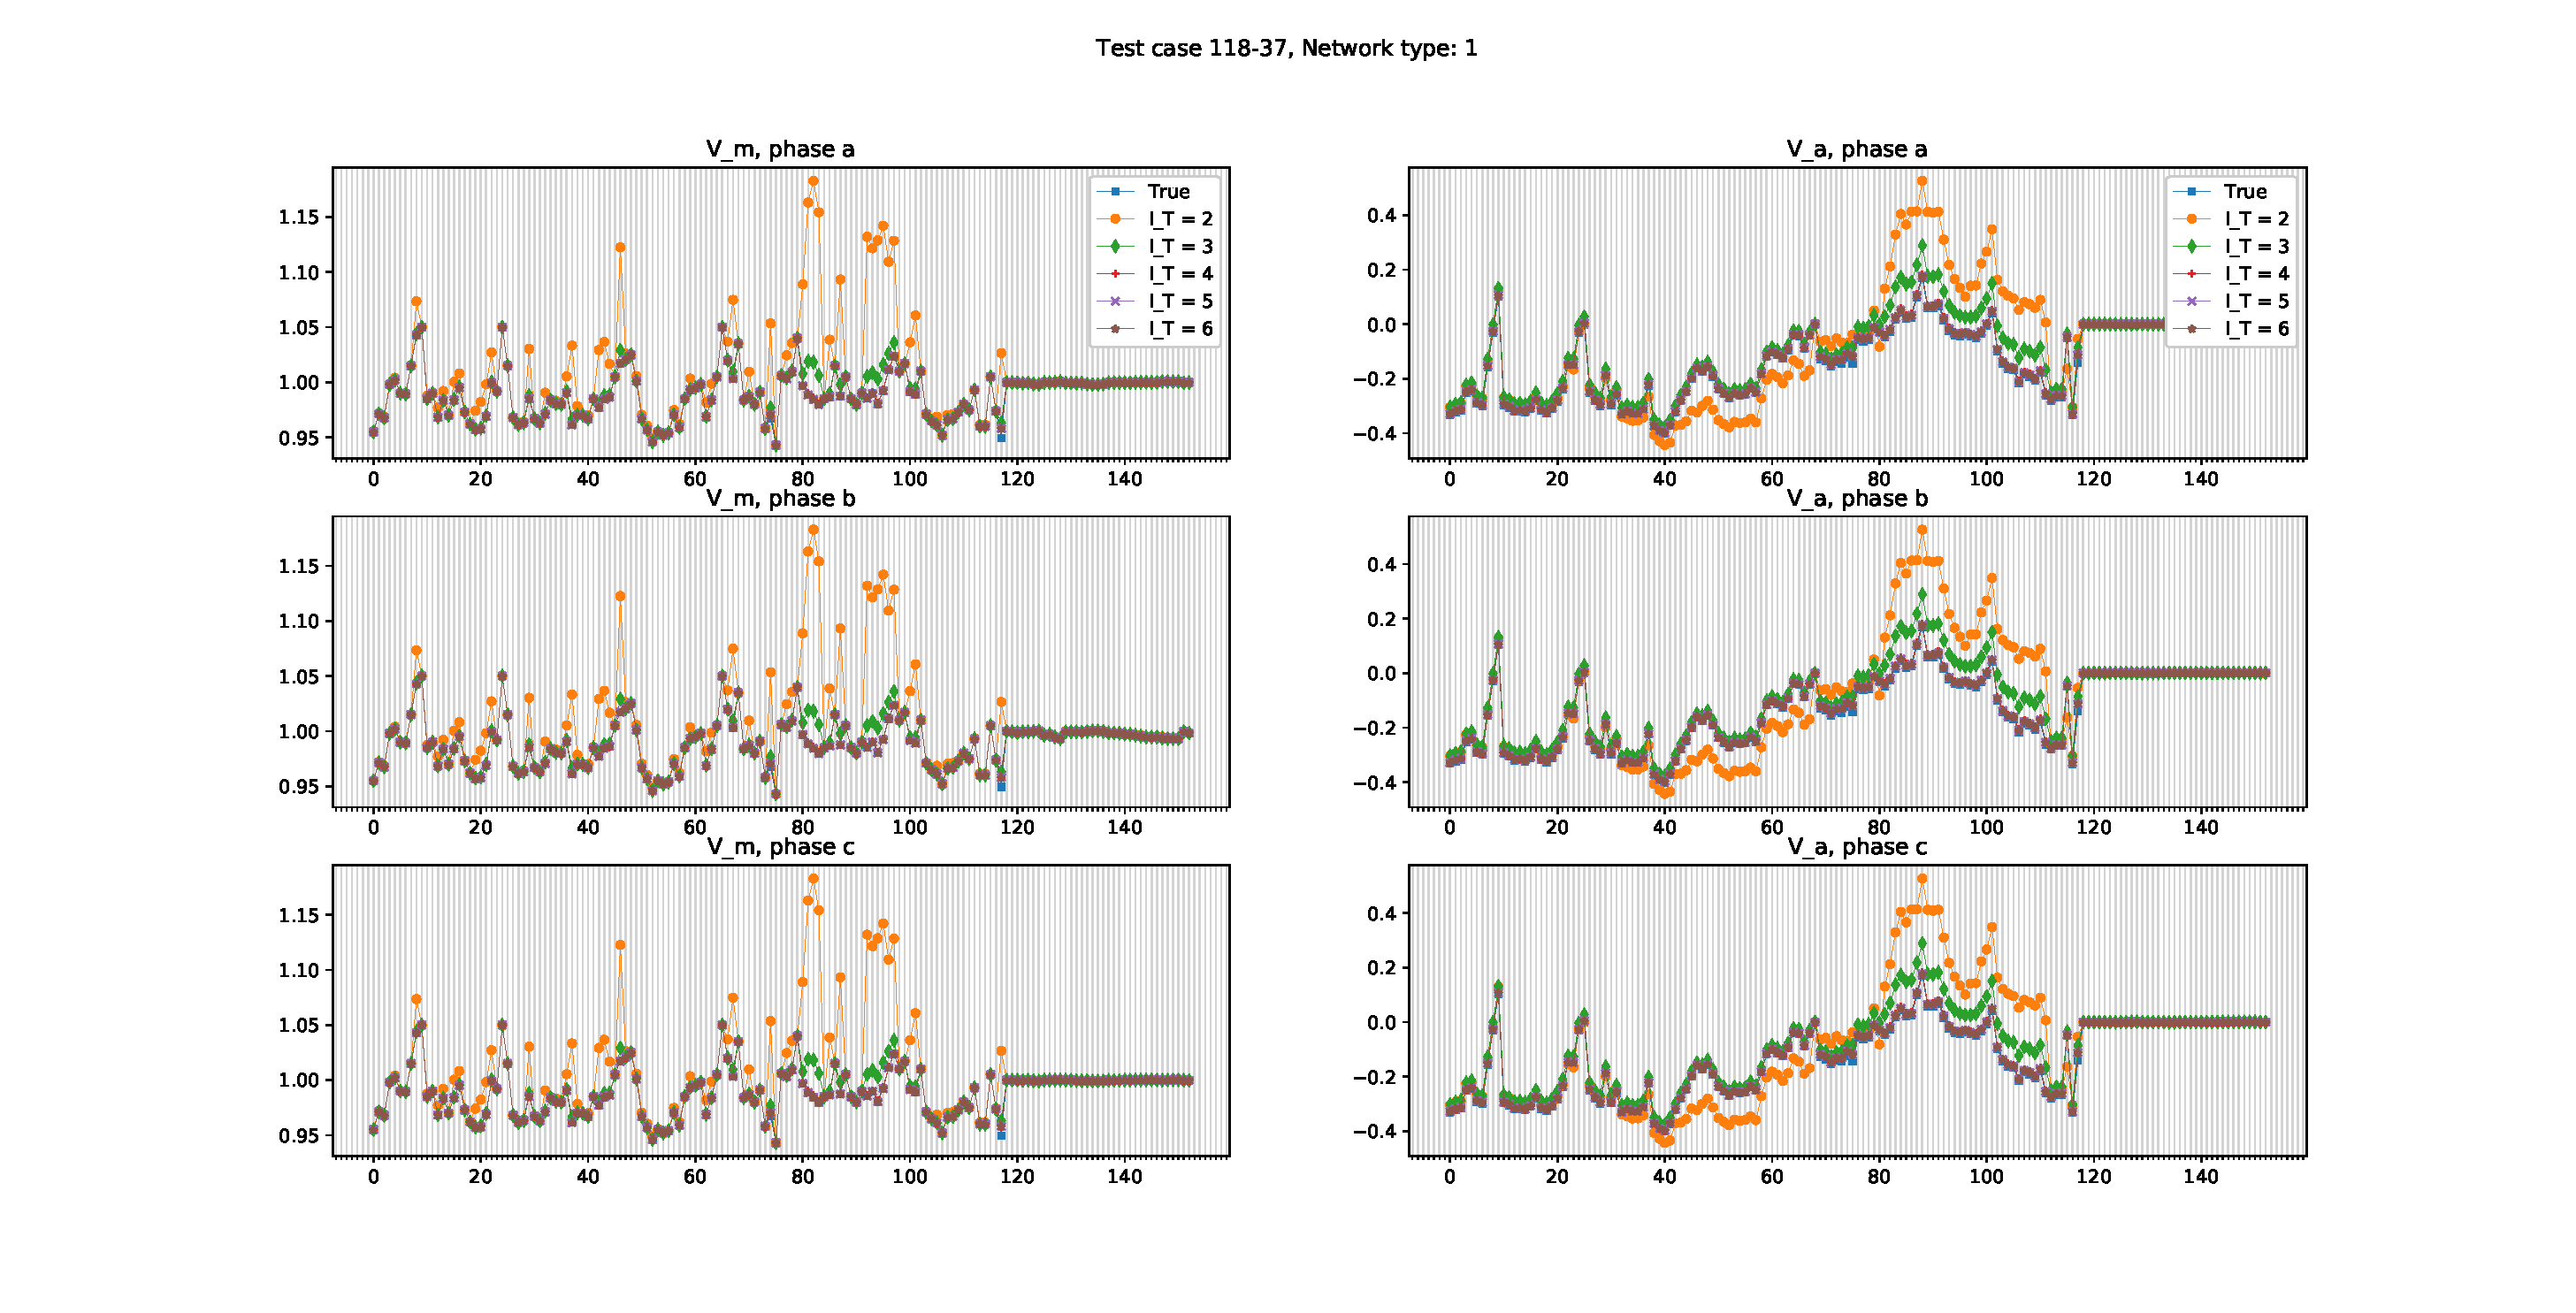
\includegraphics[width=\textwidth]{Images/MAI_N1.eps}
\caption{Voltage profile (left: magnitude, right: angle) of the MAI-schemes with increasing number of subiterations, applied on hybrid networks}\label{fig:MAIN1}
\end{figure}
\begin{figure}[!ht]
\centering
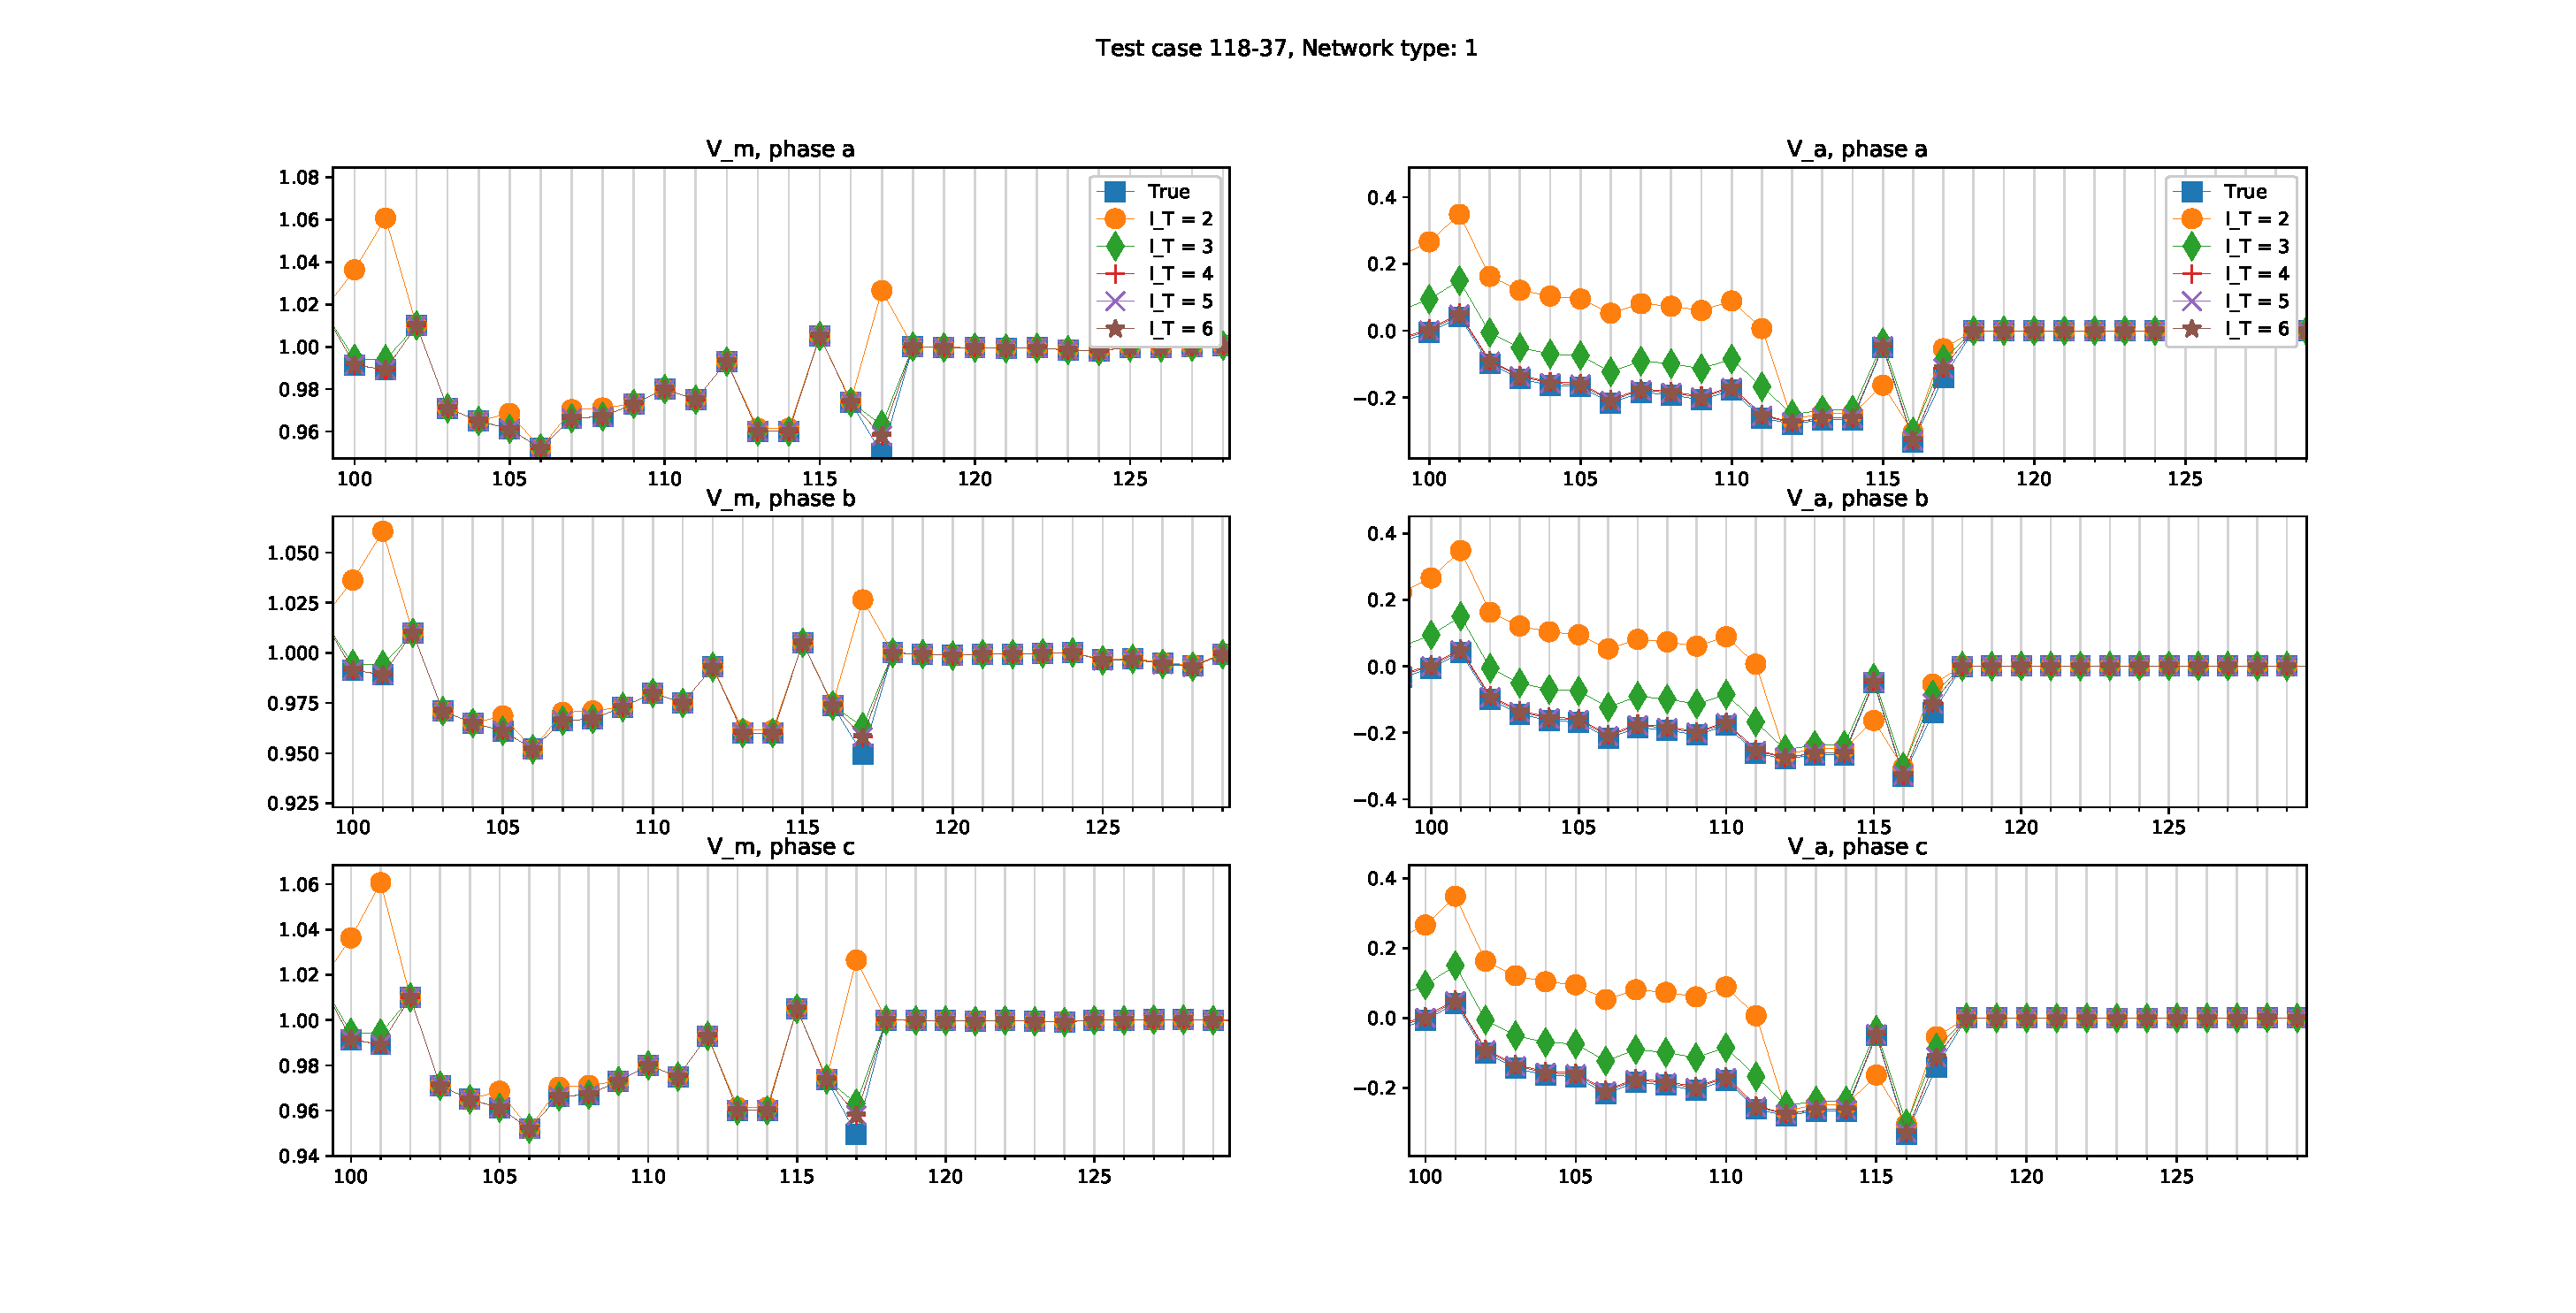
\includegraphics[width=\textwidth]{Images/Z_MAI_N1.eps}
\caption{A magnified version of the top figure of the buses surrounding the connection bus.}\label{fig:ZMAIN1}
\end{figure}


\subsubsection{Convergence and speed} 
The previous subsection shows that all the methods produce accurate results. In order to solve realistic power flow problems, which are very large electricity networks, we need insight into the speed of the problems. In this section we compare the integration methods on CPU-time and number of iterations. We share the results in table \ref{tab:speed}. 
\begin{table}[h]
\renewcommand{\arraystretch}{1.3}
\centering
\caption{Comparison on number of iterations (in case of the MSS-method ($I_{MSS}$) and the necessary iterations per subdomain ($I_T$ and $I_D$)), and CPU-time of the integration methods, applied on five test-cases. The top one are methods applied on homogeneous networks. The bottom one is applied on hybrid networks. }\label{tab:speed}
\begin{adjustbox}{width=1\textwidth} %, angle=90}
\small
\begin{tabular}{@{}l c cc c  cccc c cccc c  @{}}\toprule
                               && \multicolumn{2}{c}{\textit{F3P}} &&     \multicolumn{4}{c}{\textit{MS-homo-CAI}} && \multicolumn{4}{c}{\textit{MS-homo-MAI}} \\ \midrule 
\multicolumn{1}{l}{}        && \textit{its}      & \textit{CPU} && $I_{MSS}$      & $I_T$   &  $I_D$      & \textit{CPU}     &&$I_{MSS}$      & $I_T$   &  $I_D$      & \textit{CPU}      \\
\cmidrule{3-4}  \cmidrule{6-9}  \cmidrule{11-14}   
\multicolumn{1}{c}{test case}      && \textit{\#}       & \textit{sec} && \textit{\#}      & \textit{\#}    & \textit{\#}       & \textit{sec}     && \textit{\#}        & \textit{\#}     &  \textit{\#}       & \textit{sec}  \\
\midrule
\multicolumn{1}{c}{\textit{T9-D13 (7)}}         && 4 &\textbf{ 0.610}    && 4 & 4 & 4 &  0.237 && 6 & 2 & 2  & {0.257}\\
\multicolumn{1}{c}{\textit{T9-D37 (7)}}         && 4 & \textbf{0.587}    && 3 & 4 & 4 &  0.262 && 6 & 2 & 2  & {0.299}\\
\multicolumn{1}{c}{{\textit{T118-D13 (118)}}}   && 5 & \textbf{0.763}    && 3 & 7 & 5  & 0.324 && 4 & 2 & 2 &  0.297  \\
\multicolumn{1}{c}{{\textit{T118-D37 (118)}}}   && 5 & \textbf{0.920}    && 3 & 7 & 5  & 0.360 && 3 & 4 & 4 &  0.3253\\
\multicolumn{1}{c}{{\textit{T3120-D37 (3003)}}} && 5 & \textbf{2438}     && 3 & 6 & 4  & 1213  && 6 & 2 & 2 &  841    \\
% \multicolumn{1}{l}{\textit{T9-2D13}}       && - & - && - & -    && -       & - & -  & \textbf{-} && -   & - & - &  - && -       & -  & - & - && -       & -  & - & - \\
% \multicolumn{1}{l}{{\textit{T9-3D13}}}    && - & - && - & -    && -       & - & -  & \textbf{-} && -   & - & - &  - && -       & -  & - & - && -       & -  & - & - \\
\toprule 
\end{tabular}
\end{adjustbox}
%homogeneous
\begin{adjustbox}{width=1\textwidth} %, angle=90}
\small
\begin{tabular}{@{}l c cc c  cccc c cccc c  @{}}\toprule
                               && \multicolumn{2}{c}{\textit{IC}} &&     \multicolumn{4}{c}{\textit{MS-hybrid-CAI}} && \multicolumn{4}{c}{\textit{MS-hybrid-MAI}} \\ \midrule 
\multicolumn{1}{l}{}        && \textit{its}      & \textit{CPU} && $I_{MSS}$      & $I_T$   &  $I_D$      & \textit{CPU}     &&$I_{MSS}$      & $I_T$   &  $I_D$      & \textit{CPU}      \\
\cmidrule{3-4}  \cmidrule{6-9}  \cmidrule{11-14}   
\multicolumn{1}{c}{test case}      && \textit{\#}       & \textit{sec} && \textit{\#}      & \textit{\#}    & \textit{\#}       & \textit{sec}     && \textit{\#}        & \textit{\#}     &  \textit{\#}       & \textit{sec}  \\
\midrule
\multicolumn{1}{c}{\textit{T9-D13 (7)}}          && 4 & {0.455 } && 4      & 4  & 4 & 0.308 && 6     & 2  & 2 & 0.323  \\
\multicolumn{1}{c}{\textit{T9-D37 (7)}}          && 4 & 0.464    && 3      & 4  & 4 & 0.325 && 6     & 2  & 2 & 0.352  \\
\multicolumn{1}{c}{{\textit{T118-D13 (118)}}}    && 4 & 0.522    && 3      & 7  & 5 & 0.348 && 4     & 2  & 2 & {0.312} \\
\multicolumn{1}{c}{{\textit{T118-D37 (118)}}}    && 4 & 0.518    && 3      & 7  & 5 & 0.356 && 3     & 4  & 4 & {0.353}\\
\multicolumn{1}{c}{{\textit{T3120-D37 (3003)}}}  && 5 & 143      && 3      & 6  & 4 & 383   && 6     & 2  & 2 & {235}  \\
% \multicolumn{1}{l}{\textit{T9-2D13}}       && - & - && - & -    && -       & - & -  & \textbf{-} && -   & - & - &  - && -       & -  & - & - && -       & -  & - & - \\
% \multicolumn{1}{l}{{\textit{T9-3D13}}}    && - & - && - & -    && -       & - & -  & \textbf{-} && -   & - & - &  - && -       & -  & - & - && -       & -  & - & - \\
\toprule 
\end{tabular}
\end{adjustbox}
\end{table}
These results show that over all the test cases, the full three-phase method performs the least. The rest of the methods are comparable in speed for the small test-cases. The big test case, test-case 5, gives the most significant results. The hybrid network methods are a lot faster than the homogeneous methods. \newline \newline
There is not a clear significance in the MSS-CAI- and MAI-schemes. We would recommend to choose the CAI method as this method is only a bit slower than the MAI method, but you will always get accurate results. With the MAI-scheme, you first have to find out how many subiterations are required before convergence.  

\section{Conclusion}
We have reviewed and assessed two types of integration methods to solve the power flow problem. We classified them as unified and splitting methods and applied them on hybrid and homogeneous networks. We checked if the methods produced accurate results and analyzed the speed and number of iterations before convergence has been reached. \newline
From this assessment we can conclude that the methods applied on hybrid networks most favourable in sense of CPU-time. This can be easily argued as the size of the Jacobian in the transmission subdomain increases from having size 2n by 2n, to having a size of 6n by 6n. $n$ is the number of transmission buses. The differences between the splitting and unified methods applied on hybrid networks are less significant. We would recommend to choose the unified methods when this is possible. But in geographically distinct locations, or when legislation prohibits system operators to share complete network data, the splitting methods are very valuable. The speed of the CAI-schemes can be reduced when we apply the idea of paragraph \ref{par:caischeme}. \newline\newline
The next step is to continue with realistic test cases which can be up to millions of buses per subdomain. In most countries, the transmission network is much smaller than the distribution network and a country has most of the time more than one distribution network. The differences between homogeneous and hybrid methods become less significant. Furthermore, these very large networks must be solved in parallel which require other technique. The MSS-method has an advantage here, it is a domain-decomposition approach: multiple distribution networks can run on parallel cores. Doing new simulations using these speed-up techniques on realistically sized networks, should give a better idea which method is most favourable to solve the integrated power flow problem. 

%\section{References}
\newpage
\bibliographystyle{ieeetr}
\bibliography{pscc3} 


\end{document}
